\section{Numerical examples}
\label{Sec3:resultsDisc}
Acoustic scattering problems on a sphere are investigated in the following. These problems possess analytic solutions~\cite{Venas2019e3s} and are for this reason often used to verify numerical methods in acoustic scattering, e.g.~\cite{Gerdes1996so3,Ihlenburg1998fea,Simpson2014aib,Gerdes1998tcv,Gerdes1999otp,Coox2017aii}. In order to analyze convergence properties of IGABEM we also consider a torus, which can be represented by NURBS of polynomial order $\check{p}\geq 2$ with no poles in the parametrization. Also, a cube geometry will be investigated to check the behavior of the BIEs at $G^0$-geometries. We then continue be analyzing the BeTSSi\footnote{Benchmark Target Strength Simulation.} submarine. Before we consider the rigid scattering problem on this complex geometry, we present the method of manufactured solution. This method enables us to get some quality insurance of the underlying mesh to be used in the full scattering problem. Moreover, to some extent, the method can be used for quality insurance of the numerical solution of the scattering problem. Together with the benchmark problem on the sphere, these methods yield a solid basis for testing the correctness of the implemented code.

In this work, the test setting is chosen so that the present approach can be compared to other methods. In particular, the scattering on a rigid sphere example and the torus example is found in~\cite{Simpson2014aib}. Scattering on the BeTSSi submarine has been addressed at three workshops in the past 18 years~\cite{Nolte2014bib}. FWG\footnote{Forschungsanstalt f\"{u}r Wasserschall und Geophysik.} initiated the first workshop in 2001 (held in Kiel 2002) and delivered the generic BeTSSi submarine (for which the outer hull is described in~\Cref{Sec3:BeTSSi_description}). The second workshop took place in Kiel in 2014 and the third in the Hague in 2016. The best of these results will be used as reference solutions in this work. Additionally, we create our own reference simulations using \COMSOL~\cite{ComsolV54}. This benchmarking exercise is a crucial step to obtain reliable solutions for even more complex models.

The aim of these numerical examples is to investigate the approximability of IGABEM and its formulations. Moreover, we aim to establish highly accurate solutions for the BeTSSi submarine for benchmarking purposes and compare the accuracy and computational complexity of these results to existing simulations.

With the use of the Galerkin method the following quasi-optimal error estimate exists for the BEM~\cite[Theorem 2.49]{Chandler_Wilde2012nab} (with the Burton--Miller formulation)
\begin{equation}\label{Eq3:aprioriErrorEstimate}
	\|p-p_h\|_{L^2(\Gamma)} \leq C_1 \inf_{q_h\in V_h}\|p-q_h\|_{L^2(\Gamma)} \leq C_2 (hk)^{\check{p}+1}
\end{equation}
where $V_h$ is the finite dimensional subspace in which the solution is sought and the constants $C_1$ and $C_2$ may depend on the analytic solution $p$, the boundary $\Gamma$ and the wave number $k$. In this work we also aim to give numerical evidence for similar estimates for the other BEM formulations.

The simulations are based on the ASIGA\footnote{The ASIGA (Acoustic Scattering with IsoGeometric Analysis) library can be found at \href{https://github.com/Zetison/ASIGA}{https://github.com/Zetison/ASIGA}.} library written in \MATLAB~\cite{MatlabR2019a}. The integration is here vectorized over the quadrature points, such that the effect of increasing the number of quadrature points is of less significance due to the efficiency of vectorization in \MATLAB. For this reason, we take the liberty of over integration the BIEs without suffering to much from computational cost. For optimization purposes, the library could be written in \ccpp which would require an accuracy-cost tradeoff study in this respect. Additionally, acceleration techniques exist for the boundary element method which have not been implemented in the ASIGA library. We refer to \cite{Dolz2016aib,Dolz2018afi,Beer2008tbe} for details. These optimizations are suggested as future work.

The BIE formulations listed in~\Cref{Tab3:BIEs} will be investigated both in terms of approximability and the presence of fictitious eigenfrequencies.
\begin{table}
	\centering
	\caption{Overview of the boundary integral equation (BIE) formulations considered in this work.}
	\label{Tab3:BIEs}
	\begin{tabular}{l l l}
		\toprule
		Abbreviation & Name & Definition\\
		\hline
		CBIE & Conventional BIE & \Cref{Eq3:CBIE}\\
		RCBIE$i$ & The $i^{\mathrm{th}}$ regularized CBIE & \Cref{Eq3:RCBIE1,Eq3:RCBIE2,Eq3:RCBIE3}\\
%		RCBIE1 & The first regularized CBIE & \Cref{Eq3:RCBIE1}\\
%		RCBIE2 & The second regularized CBIE & \Cref{Eq3:RCBIE2}\\
%		RCBIE3 & The third regularized CBIE & \Cref{Eq3:RCBIE3}\\
		HBIE & Hypersingular BIE & \Cref{Eq3:HBIE}\\
		BM & Burton--Miller & \Cref{Eq3:BM}\\
		\bottomrule
	\end{tabular}
\end{table}

The meshes will be generated from a coarse CAD model mesh (for example \Cref{Fig3:parm1} for the sphere) with mesh number $m=1$. We shall denote by ${\cal M}_{m,\check{p},\check{k}}^{\textsc{igabem}}$, mesh number $m$ with polynomial order $\check{p}$ and continuity $\check{k}$ across element boundaries\footnote{Except for (potentially) some $C^0$ lines in the initial CAD geometry.}. For the corresponding FEM meshes we denote by ${\cal M}_{m,\check{p},\mathrm{s}}^{\textsc{fembem}}$ and ${\cal M}_{m,\check{p},\mathrm{i}}^{\textsc{fembem}}$ the subparametric and isoparametric FEM meshes, respectively. These meshes are constructed by the procedure outlined in~\cite[p. 191]{Venas2018iao}.

\subsection{Pulsating sphere}
\label{Sec3:pulsatingSphere}
Consider a pulsating unit sphere centered at the origin (cf. \cite{Simpson2014aib,Zheng2015itb}) with analytic solution given by
\begin{equation}
	p(\vec{x}) = \frac{\euler^{\imag kR}}{4\PI R},\quad R=|\vec{x}|,\quad \vec{x}\in\Omega^+
\end{equation}
and with the (constant) Neumann condition
\begin{equation}
	g(\vec{x}) = \frac{\euler^{\imag k}}{4\PI}(\imag k -1),\quad \vec{x}\in\Gamma.
\end{equation}
This problem serves as a patch test for IGA as the analytic solution lies in the numerical solution space ($p(\vec{x})$ is constant at $\Gamma$). Contrary to FEM with affine mappings, (proper) Gaussian quadrature does not integrate the integrals in BEM exactly. Therefore, this example may be used to give some indication of the quality of the integration procedure. In~\Cref{Fig3:Simpson_PS_1,Fig3:Simpson_PS_2} we compare the two adaptive quadrature schemes (described in~\Cref{Sec3:numericalQuad}), where we set $n_{\mathrm{eqp},2}=100$ to avoid error originating from the integration over the element containing the source points. The $L^2$-error of the numerical solution is here plotted against $n_{\mathrm{qp},1}$; the total number of quadrature points, excluding quadrature points in elements containing the source point. The simulations are done on the coarsest mesh of the second NURBS parametrization in~\Cref{Fig3:parm2} (with $\check{p}=4$). The BM and HBIE formulations (for both collocation and Galerkin) have more round-off errors and are for this reason further away from machine epsilon precision results compared to the other formulations. In all cases, the new adaptive quadrature scheme obtains better results. Interestingly CBIE obtains slightly better results using the new adaptive quadrature scheme compared to RCBIE3, the latter being the regularized version of the former. This might be due to the reduction of symmetry in the RCBIE3 compared to CBIE for this problem.

\begin{figure}
	\begin{subfigure}{0.49\textwidth}
		\centering
		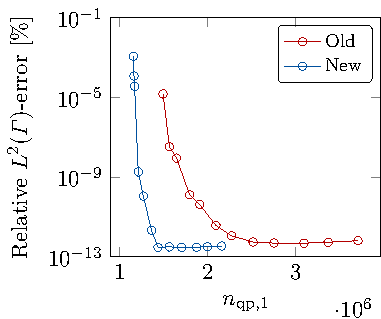
\includegraphics[width=0.8\textwidth]{Simpson_PS_1}
		\caption{CCBIE}
	\end{subfigure}%
	\hspace*{0.02\textwidth}%
	\begin{subfigure}{0.49\textwidth}
		\centering
		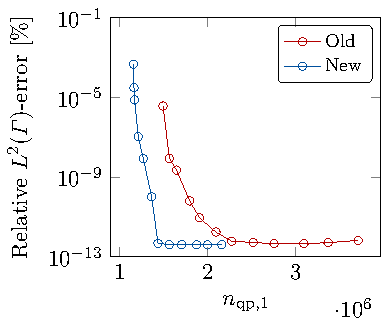
\includegraphics[width=0.8\textwidth]{Simpson_PS_2}
		\caption{CRCBIE3}
	\end{subfigure}
	\par\bigskip
	\par\bigskip
	\begin{subfigure}{0.49\textwidth}
		\centering
		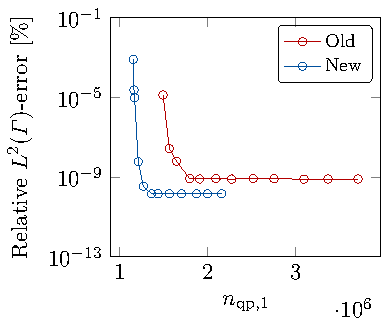
\includegraphics[width=0.8\textwidth]{Simpson_PS_7}
		\caption{CHBIE}
	\end{subfigure}%
	\hspace*{0.02\textwidth}%
	\begin{subfigure}{0.49\textwidth}
		\centering
		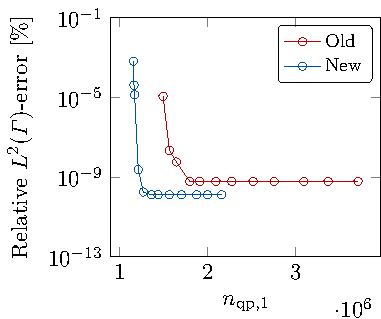
\includegraphics[width=0.8\textwidth]{Simpson_PS_8}
		\caption{CBM}
	\end{subfigure}
	\par\bigskip
	\par\bigskip
	\begin{subfigure}{0.49\textwidth}
		\centering
		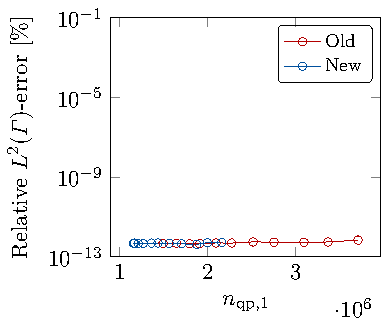
\includegraphics[width=0.8\textwidth]{Simpson_PS_13}
		\caption{CRCBIE1}
	\end{subfigure}%
	\hspace*{0.02\textwidth}%
	\begin{subfigure}{0.49\textwidth}
		\centering
		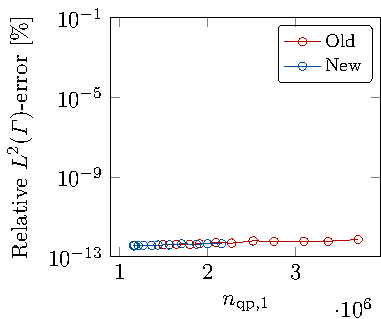
\includegraphics[width=0.8\textwidth]{Simpson_PS_14}
		\caption{CRCBIE2}
	\end{subfigure}
	\caption{\textbf{Pulsating sphere}: Surface error as a function of the total number of quadrature points $n_{\mathrm{qp,1}}$ at $kR_0=1$.  The old adaptive quadrature scheme presented by Simpson in~\cite{Simpson2014aib} is compared to the new adaptive quadrature scheme presented in this work. The sample points correspond to $s_1\in\{1,2,\dots,12\}$ and $s_1\in\{1,2,\dots,12\}/5$ for the old and new method, respectively.}
	\label{Fig3:Simpson_PS_1}
\end{figure}
Note that for this problem using RCBIE1 or RCBIE2 (\Cref{Eq3:RCBIE1,Eq3:RCBIE2}), results with machine epsilon precision are always obtained since the integrands are zero. This is due to the spherical symmetry of the problem and the functions involved.

\begin{figure}
	\begin{subfigure}{0.49\textwidth}
		\centering
		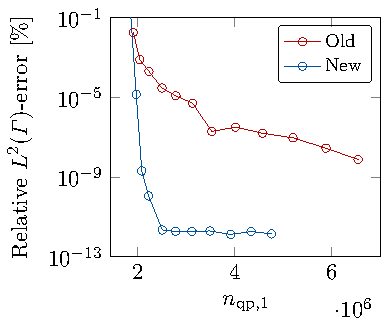
\includegraphics[width=0.8\textwidth]{Simpson_PS_5}
		\caption{GCBIE}
	\end{subfigure}%
	\hspace*{0.02\textwidth}%
	\begin{subfigure}{0.49\textwidth}
		\centering
		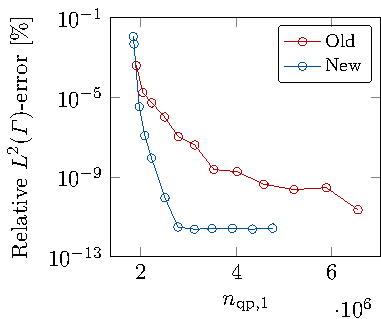
\includegraphics[width=0.8\textwidth]{Simpson_PS_6}
		\caption{GRCBIE3}
	\end{subfigure}
	\par\bigskip
	\par\bigskip
	\begin{subfigure}{0.49\textwidth}
		\centering
		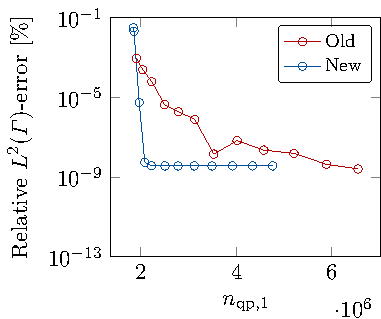
\includegraphics[width=0.8\textwidth]{Simpson_PS_11}
		\caption{GHBIE}
	\end{subfigure}%
	\hspace*{0.02\textwidth}%
	\begin{subfigure}{0.49\textwidth}
		\centering
		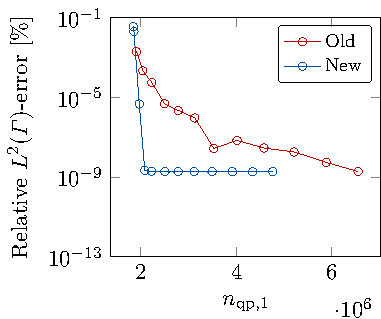
\includegraphics[width=0.8\textwidth]{Simpson_PS_12}
		\caption{GBM}
	\end{subfigure}
	\par\bigskip
	\par\bigskip
	\begin{subfigure}{0.49\textwidth}
		\centering
		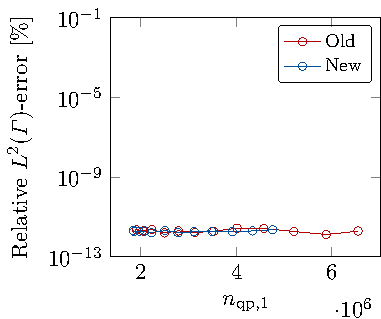
\includegraphics[width=0.8\textwidth]{Simpson_PS_17}
		\caption{GRCBIE1}
	\end{subfigure}%
	\hspace*{0.02\textwidth}%
	\begin{subfigure}{0.49\textwidth}
		\centering
		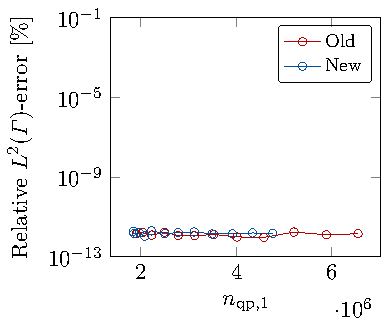
\includegraphics[width=0.8\textwidth]{Simpson_PS_18}
		\caption{GRCBIE2}
	\end{subfigure}
	\caption{\textbf{Pulsating sphere}: Surface error as a function of the total number of quadrature points $n_{\mathrm{qp,1}}$ at $kR_0=1$.  The old adaptive quadrature scheme presented by Simpson in~\cite{Simpson2014aib} is compared to the new adaptive quadrature scheme presented in this work. The sample points correspond to $s_1\in\{1,2,\dots,12\}$ and $s_1\in\{1,2,\dots,12\}/5$ for the old and new method, respectively.}
	\label{Fig3:Simpson_PS_2}
\end{figure}
Based on this study, a proper choice for the parameter $s_1$ is $s_1=1.4$ for the new adaptive method. If not otherwise stated, we shall use $s_1=1.4$ and $n_{\mathrm{eqp},2}=50$, which in most cases results in over integration. As was mentioned before, the cost of this is not significant due to the current implementation in \MATLAB.

\subsection{Rigid scattering on a sphere} 
Consider a plane wave, with the direction of incidence given by
\begin{equation}\label{Eq3:d_s}
	\vec{d}_{\mathrm{s}} = -\begin{bmatrix}
		\cos\beta_{\mathrm{s}}\cos\alpha_{\mathrm{s}}\\
		\cos\beta_{\mathrm{s}}\sin\alpha_{\mathrm{s}}\\
		\sin\beta_{\mathrm{s}}
	\end{bmatrix},
\end{equation}
with\footnote{The angles $\alpha$ and $\beta$ are the so-called aspect and elevation angle, respectively. Note that the aspect angle is equal to the spherical coordinate $\varphi$ (the azimuth angle).} $\alpha_{\mathrm{s}} = \ang{240}$ and $\beta_{\mathrm{s}} = \ang{30}$, scattered by a rigid sphere with radius $R_0=\SI{1}{m}$. 
\begin{figure}
	\centering
	\begin{subfigure}[t]{0.3\textwidth}
		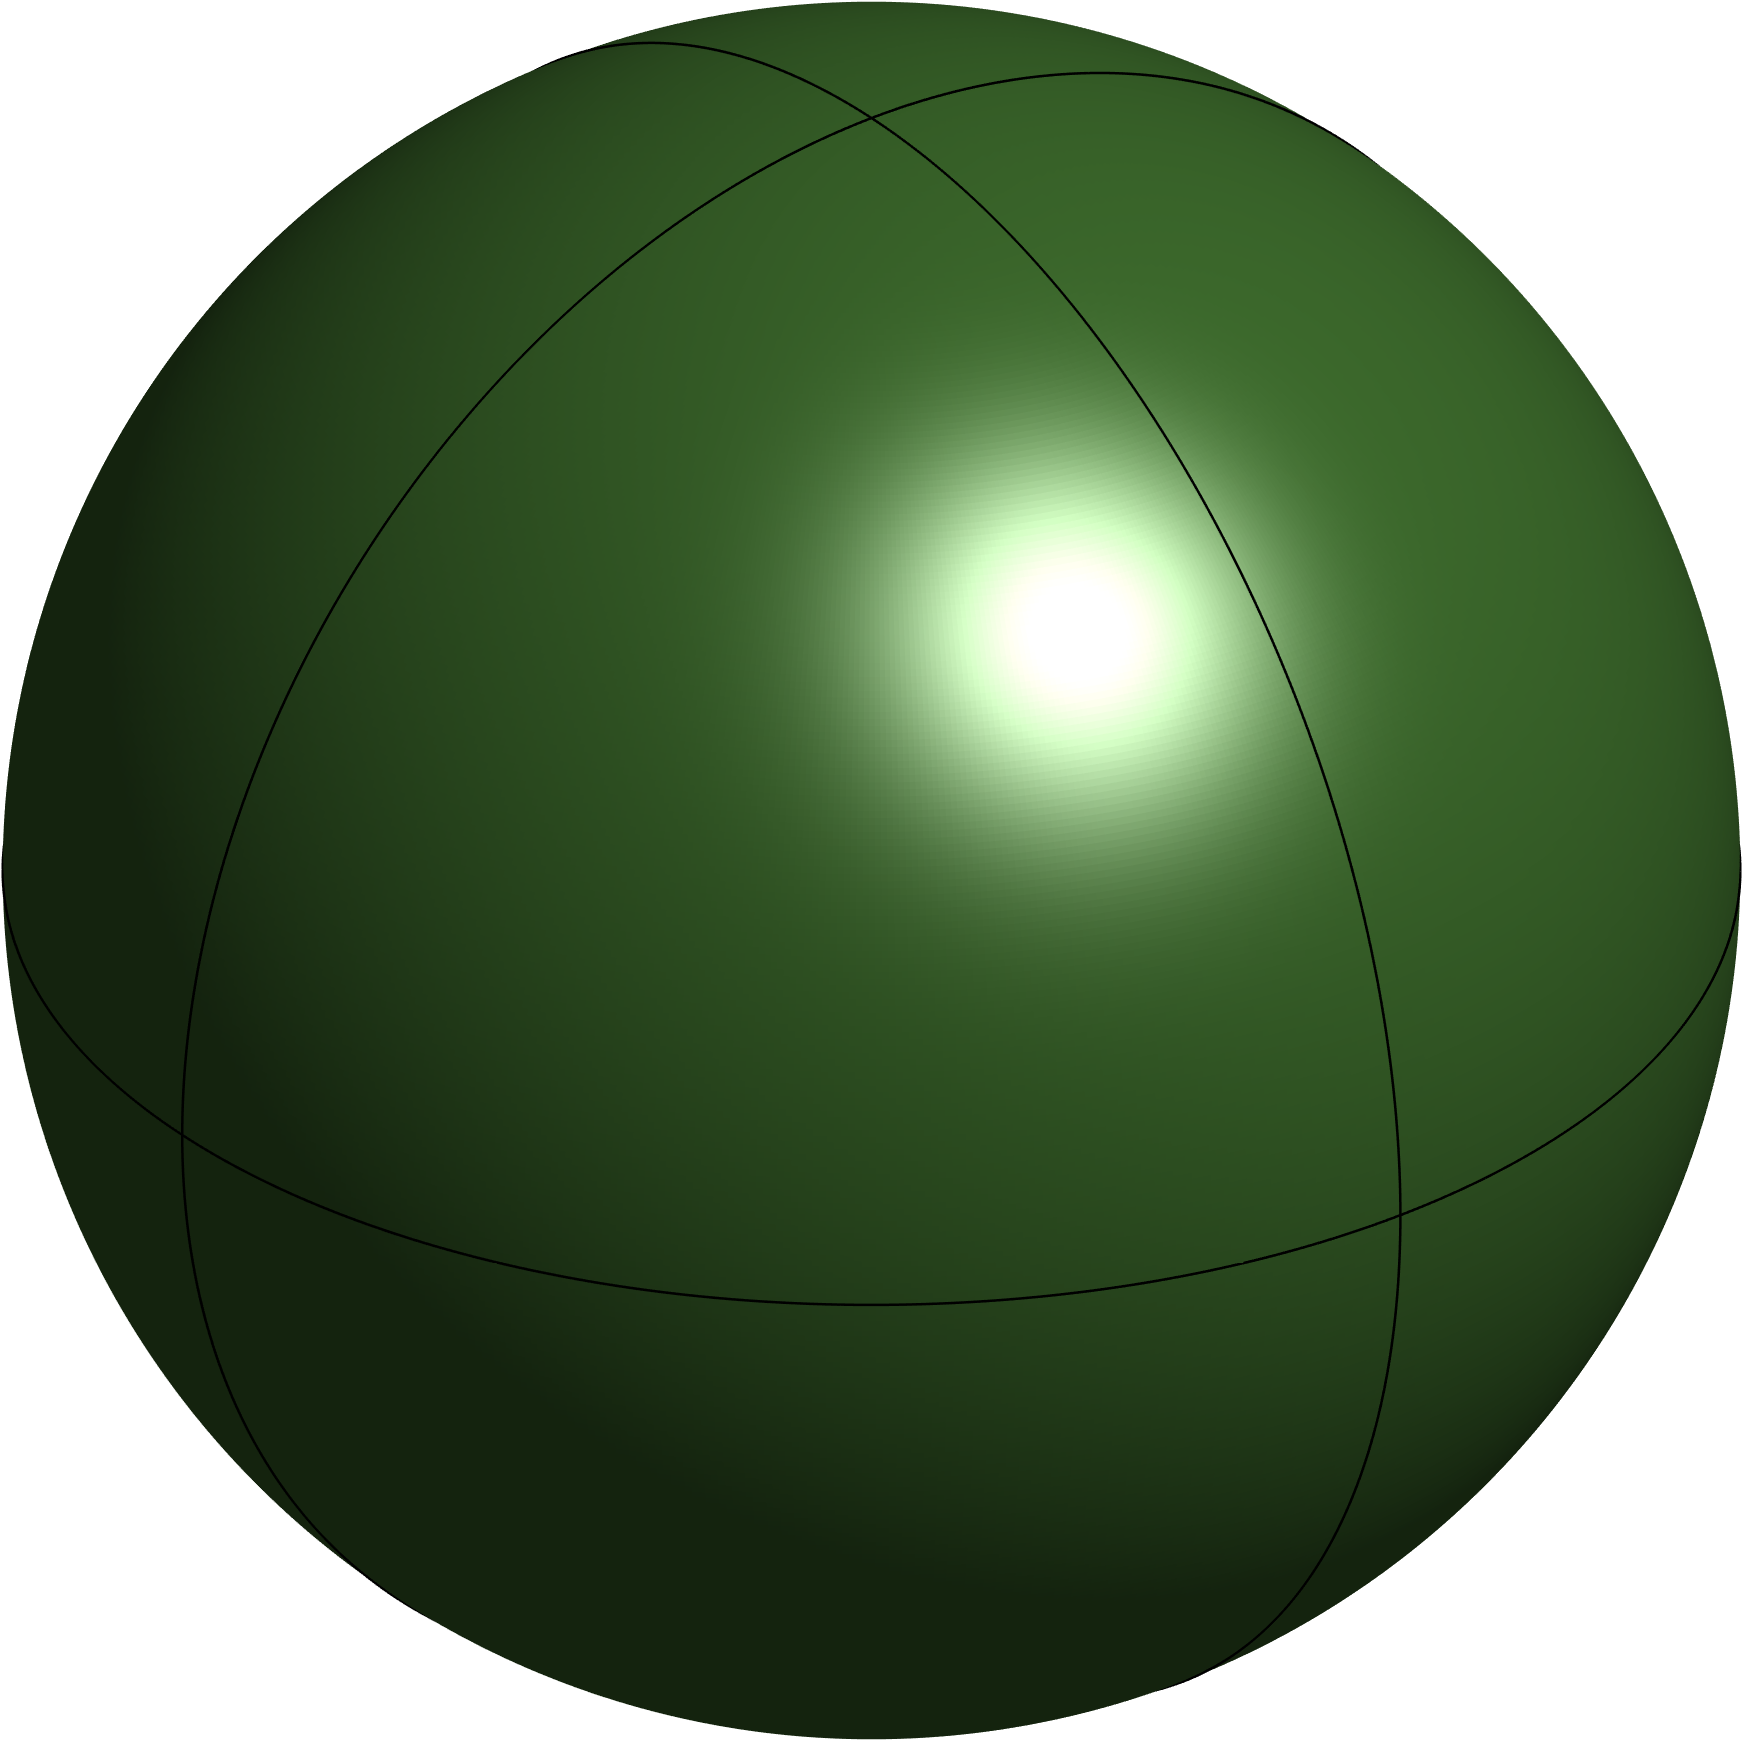
\includegraphics[width=0.9\textwidth]{sphericalShellMesh1_2_0}
		\caption{Parametrization 1.}
		\label{Fig3:parm1}
	\end{subfigure} 
	~
	\begin{subfigure}[t]{0.3\textwidth}
		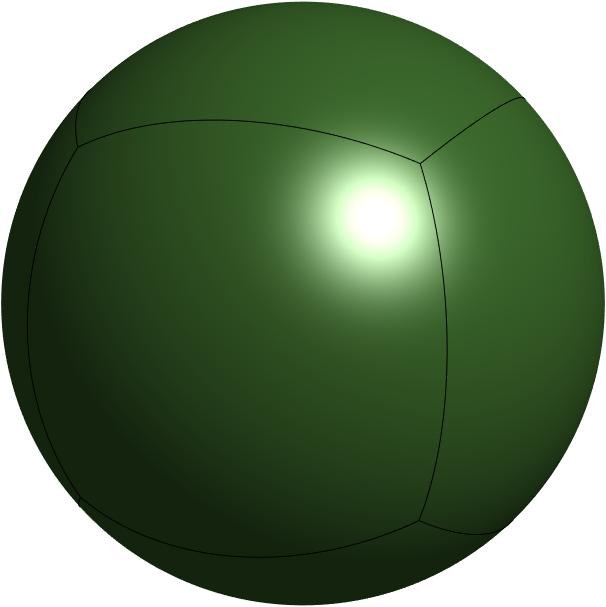
\includegraphics[width=0.9\textwidth]{patchedShellMesh1}
		\caption{Parametrization 2.}
		\label{Fig3:parm2}
	\end{subfigure} 
	\caption{Two exact NURBS parametrizations of the sphere. Parametrization 1 uses a single patch with 8 elements of degree $\check{p}\geq 2$ while parametrization 2 uses 6 patches of degree $\check{p}\geq 4$. Parametrization 1 is described in~\Cref{Sec3:NURBSsphere1} and parametrization 2 is described in \Cref{Sec3:NURBSsphere2}.}
	\label{Fig3:SphericalShellParametrizations}
\end{figure}

For the rigid scattering problems considered in this work, the error is computed of $p_{\mathrm{tot}}$ and the best approximation (BA) is obtained by performing an $L^2$-projection of $p_{\mathrm{tot}}$ onto the discretized solution space. 

Continuing the study of numerical quadrature, we investigate the parameters $s_1$ and $n_{\mathrm{eqp},2}$ also for rigid scattering. The study for the parameter $s_1$ uses $n_{\mathrm{eqp},2}=100$ and the study for $n_{\mathrm{eqp},2}$ uses $s_1=0.7$. 

For FEM/IGA using $\check{p}+1$ quadrature points in each parametric direction in each element ensures accurate numerical integration regardless of the computational mesh. As can be observed from \Cref{Fig3:S1_qp_M5p2,Fig3:S1_qp_M4p5,Fig3:S1_qp_M5p5} this is not the case for BEM. Separate choices for the parameters $n_{\mathrm{eqp},2}$ and $s_1$ need to be made for each formulation. 

Contrary to FEM/IGA, the optimal quadrature rule seems to be depending on $h$-refinement (not only $\check{p}$-refinement). Although the integrals in the CBIE formulation are regularized to contain no singular integrals, the parameter $s_1$ may still not be set to zero. This could be expected due to the gradients around the source points.

\begin{figure}
	\centering    
	\begin{subfigure}[t]{0.49\textwidth}
		\centering
		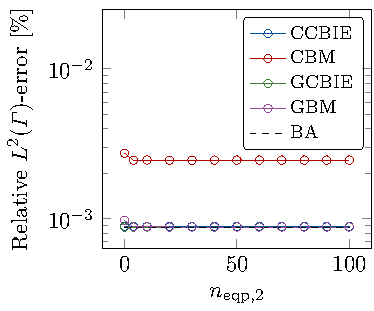
\includegraphics{S1_qp_1}
	\end{subfigure}%
	\hspace*{0.02\textwidth}%
	\begin{subfigure}[t]{0.49\textwidth}
		\centering
		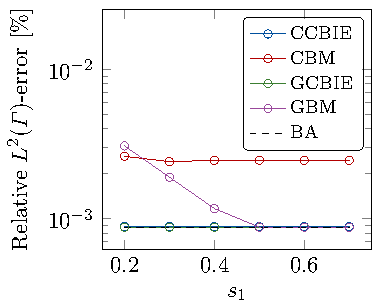
\includegraphics{S1_qp_2}
	\end{subfigure}
	\caption{\textbf{Rigid scattering on a sphere}: Surface error as a function of the parameters $n_{\mathrm{eqp},2}$ and $s_1$ to the left and right, respectively, on the mesh ${\cal M}_{5,2,1}^{\textsc{igabem}}$.}
	\label{Fig3:S1_qp_M5p2}
\end{figure}
\begin{figure}
	\centering
	\begin{subfigure}[t]{0.49\textwidth}
		\centering
		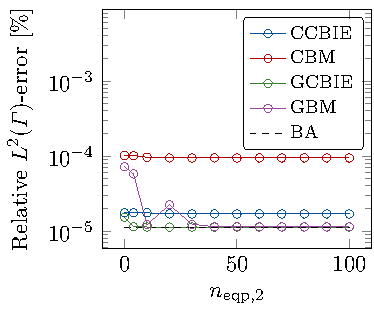
\includegraphics{S1_qp_3}
	\end{subfigure}%
	\hspace*{0.02\textwidth}%
	\begin{subfigure}[t]{0.49\textwidth}
		\centering
		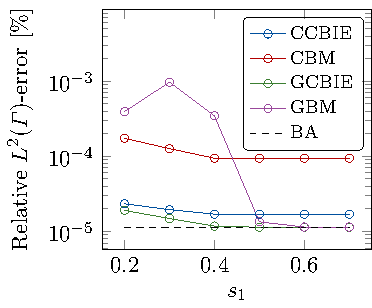
\includegraphics{S1_qp_4}
	\end{subfigure}
	\caption{\textbf{Rigid scattering on a sphere}: Surface error as a function of the parameters $n_{\mathrm{eqp},2}$ and $s_1$ to the left and right, respectively, on the mesh ${\cal M}_{4,5,4}^{\textsc{igabem}}$.}
	\label{Fig3:S1_qp_M4p5}
\end{figure}
\begin{figure}
	\centering
	\begin{subfigure}[t]{0.49\textwidth}
		\centering
		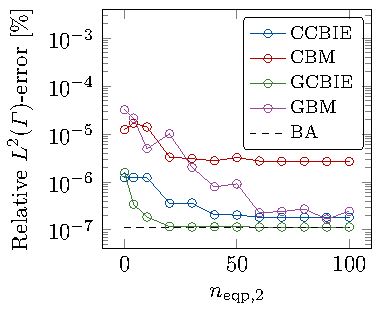
\includegraphics{S1_qp_5}
	\end{subfigure}%
	\hspace*{0.02\textwidth}%
	\begin{subfigure}[t]{0.49\textwidth}
		\centering
		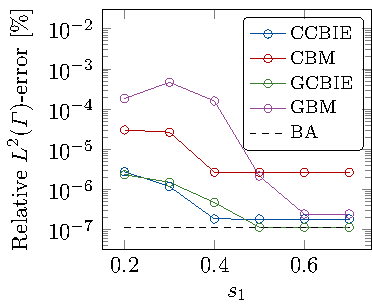
\includegraphics{S1_qp_6}
	\end{subfigure}
	\caption{\textbf{Rigid scattering on a sphere}: Surface error as a function of the parameters $n_{\mathrm{eqp},2}$ and $s_1$ to the left and right, respectively, on the mesh ${\cal M}_{5,5,4}^{\textsc{igabem}}$.}
	\label{Fig3:S1_qp_M5p5}
\end{figure}

For convenience we perturb the collocation points at the north and the south pole of the parametrization in \Cref{Fig3:parm1} in the HBIE and BM formulation for the ease of implementation. The perturbation is taken to be a distance $\frac12|\Diff\eta_e|/\check{p}_\upeta$ in the $\eta$-direction (in the parametric space), where $|\Diff\eta_e|$ is the element interval in the parametric domain in the $\eta$-direction. A similar strategy will be employed for the corresponding problematic areas on the BeTSSi submarine. This may be a sub optimal placement of collocation points, and as we can see from \Cref{Fig3:S1parmCompC}, the CBM formulation does not obtain the accuracy of the Galerkin formulation (\Cref{Fig3:S1parmCompG}). But this is also true for parametrization 2 (which contains no poles), and so this calls for an investigation of better placement of collocation points in general for the CHBIE and CBM than that of the Greville abscissae. The CBM formulation for parametrization 1 is visibly polluted by round-off errors similar to those seen in \Cref{Sec3:pulsatingSphere}.
\begin{figure}
	\centering
	\begin{subfigure}[t]{\textwidth}
		\centering
		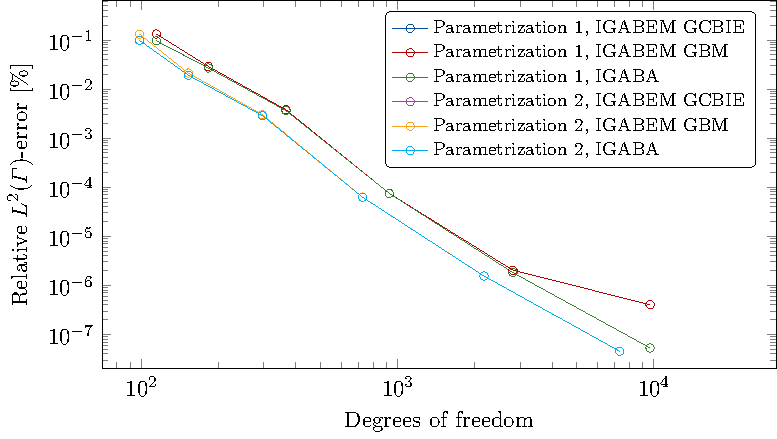
\includegraphics[width=\textwidth]{L2normPlots}
		\caption{Galerkin formulations}
		\label{Fig3:S1parmCompG}
	\end{subfigure}
	\par\bigskip
	\par\bigskip
	\begin{subfigure}[t]{\textwidth}
		\centering
		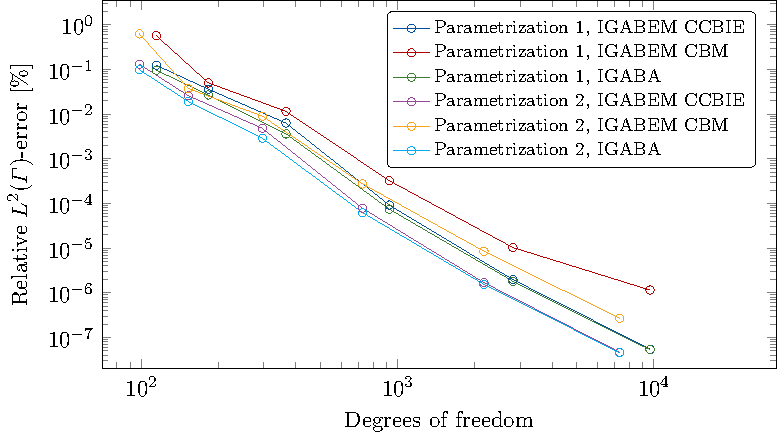
\includegraphics[width=\textwidth]{L2normPlots_C}
		\caption{Collocation formulations}
		\label{Fig3:S1parmCompC}
	\end{subfigure}
	\caption{\textbf{Rigid scattering on a sphere}: Convergence analysis with $\check{p}=4$ and $kR_0=1$.}
	\label{Fig3:S1parmComp}
\end{figure}

In~\Cref{Fig3:S1_cgComp} we can observe that CBM loses one order of convergence for the odd degree $\check{p}=3$, which is similar to the effect discussed in~\cite{Gomez2016tvc}. However, this effect does not come into play in the same way for the CCBIE formulation, although it is still a significant difference between this simulation and the best approximation. This is in stark contrast to the CCBIE simulations of even degree which approaches the best approximation solution.
\begin{figure}
	\centering
	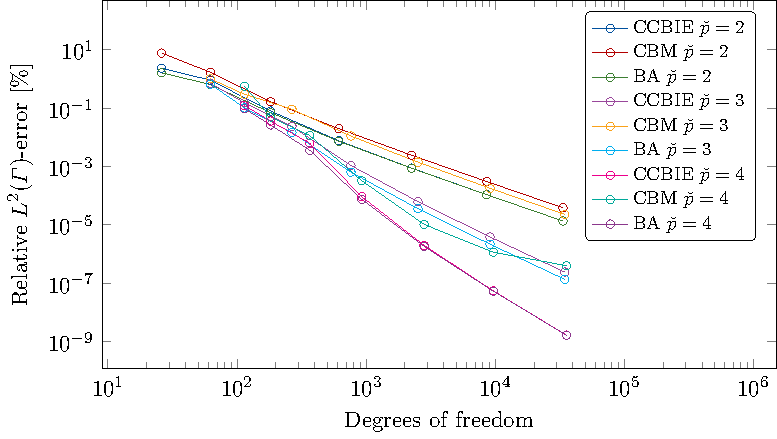
\includegraphics{L2normPlots_3}
	\caption{\textbf{Rigid scattering on a sphere}: Convergence analysis with $kR_0=1$.}
	\label{Fig3:S1_cgComp}
\end{figure}

The plots in \Cref{Fig3:S1parmComp} also show the impact a sub optimal parametrization may have. Parametrization 1 has roughly 8\% higher errors compared to parametrization 2 in terms of degrees of freedom.

In \Cref{Fig3:convergenceAnalysis} we compare the classical boundary element method (FEMBEM) with IGA. For the subparametric second order FEMBEM mesh a full convergence order (see \Cref{Fig3:convergenceAnalysis_nepw}) is lost in comparison with the best approximation for the same mesh (FEMBA). In fact, little is to be gained by increasing the polynomial order when using a linear approximation of the geometry. The exactness of the geometry is of less importance for isoparametric FEMBEM, which can be observed by comparing the results for mesh ${\cal M}_{m,2,\mathrm{i}}^{\textsc{fembem}}$ and mesh ${\cal M}_{m,2,0}^{\textsc{igabem}}$. Increasing the continuity ($\check{k}$-refinement) of the basis functions, however, improves the accuracy significantly as obtained for infinite isogeometric finite elements~\cite{Venas2018iao}.
\begin{figure}
	\centering
	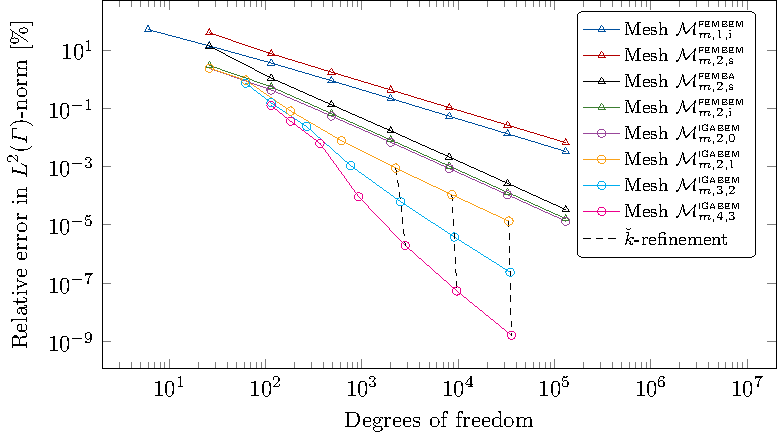
\includegraphics[width=\textwidth]{L2normPlots_24}
	\caption{\textbf{Rigid scattering on a sphere}: Convergence analysis with the CCBIE formulation on parametrization 1 for $kR_0=1$.}
	\label{Fig3:convergenceAnalysis}
\end{figure}
\begin{figure}
	\centering
	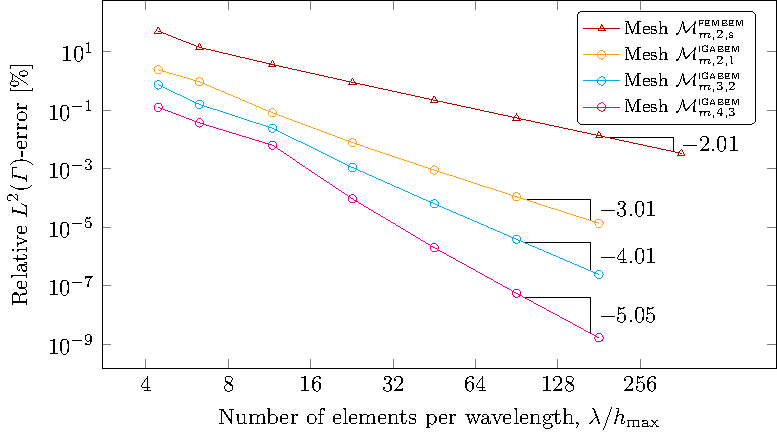
\includegraphics[width=\textwidth]{L2normPlots_1}
	\caption{\textbf{Rigid scattering on a sphere}: Convergence analysis with the CCBIE formulation on parametrization 1 for $kR_0=1$.}
	\label{Fig3:convergenceAnalysis_nepw}
\end{figure}


\begin{figure}
	\centering
	\begin{subfigure}[t]{\textwidth}
		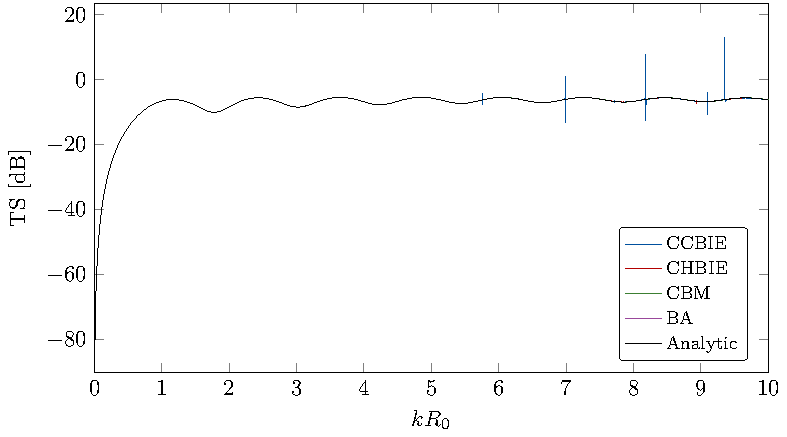
\includegraphics[width=\textwidth]{S1_sweep_TS}
		\caption{Target strength of backscattered far field.}
		\label{Fig3:eigenFreqDirichlet}
	\end{subfigure} 
	\par\bigskip
	\par\bigskip
	\begin{subfigure}[t]{\textwidth}
		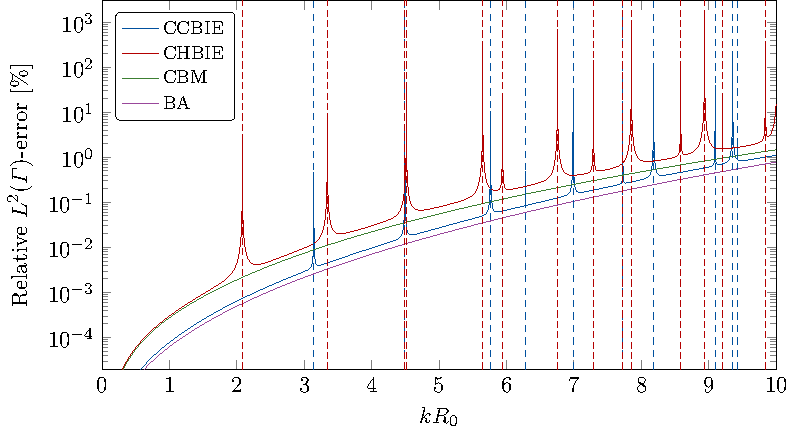
\includegraphics[width=\textwidth]{S1_sweep_surfaceError}
		\caption{Surface error on $\Gamma$.}
		\label{Fig3:eigenFreqDirichletError}
	\end{subfigure} 
	\caption{\textbf{Rigid scattering on a sphere}: The plots show the instabilities around eigenfrequencies of the corresponding interior Dirichlet problem. All computations are done using the parametrization in \Cref{Fig3:parm2} refined uniformly three times with NURBS degree 4 (resulting in 384 elements and 728 degrees of freedom).}
\end{figure}

\begin{table}
	\centering
	\caption{The non-zero dimensionless eigenvalues below $kR_0=10$ for the interior Dirichlet problem~\cite{Zheng2015itb}.}
	\label{Tab3:eigenFreqDirichlet}
	\begin{tabular}{c l}
		\toprule
		$n$ & Roots of $\besselj_n(kR_0)$ \\
		\hline
		0 & $\PI$, $2\PI$, $3\PI$, \dots \\
	    1 & 4.49340945790907, 7.72525183693771, \dots \\
	  	2 & 5.76345919689455, 9.09501133047635, \dots \\
	    3 & 6.98793200050052, \dots \\
	    4 & 8.18256145257124, \dots \\
	    5 & 9.35581211104275, \dots \\
		\bottomrule
	\end{tabular}
\end{table}
\begin{table}
	\centering
	\caption{The non-zero dimensionless eigenvalues below $kR_0=10$ for the interior Neumann problem~\cite{Zheng2015itb}.}
	\label{Tab3:eigenFreqNeumann}
	\begin{tabular}{c l}
		\toprule
		$n$ & Roots of $\besselj_n'(kR_0)$\\
		\hline
		0 & 4.49340945790907, 7.72525183693771, \dots \\
	    1 & 2.08157597781810, 5.94036999057271, 9.20584014293667, \dots \\
	  	2 & 3.34209365736570, 7.28993230409335, \dots \\
	    3 & 4.51409964703228, 8.58375495636577, \dots \\
	    4 & 5.64670362043680, 9.84044604304014, \dots \\
	    5 & 6.75645633020413, \dots \\
	    6 & 7.85107767947440, \dots \\
	    7 & 8.93483887835284, \dots \\
		\bottomrule
	\end{tabular}
\end{table}

As we can see from \Cref{Fig3:eigenFreqDirichlet}, the dimensionless fictitious eigenfrequencies in \Cref{Tab3:eigenFreqDirichlet,Tab3:eigenFreqNeumann} appear quite clearly for the CBIE and the HBIE, respectively, while the eigenvalues for the Burton--Miller formulation are shifted away from the real axis into the complex plane \cite{Zheng2015itb}. The fictitious eigenfrequencies are of course not present in the best approximation (BA) solution.

\subsection{Torus interior acoustic problem}
Consider the Torus problem presented in~\cite{Simpson2014aib}. This example sets the stage for optimal conditions for the a priori error estimate in~\Cref{Eq3:aprioriErrorEstimate} to be fulfilled. The geometry of the torus (with parametrization described in~\Cref{Sec3:torus}) has $G^\infty$ continuity and contains no polar singularities in the exact NURBS parametrization illustrated in~\Cref{Fig3:Torus} (as opposed to the sphere parametrization in~\Cref{Fig3:parm1}). The torus considered here has major radius $r_{\mathrm{o}} = 2$ and minor radius $r_{\mathrm{i}}=1$. 

Consider the exact solution
\begin{equation*}
	p(\vec{x}) = \sin\frac{kx_1}{\sqrt{3}}\sin\frac{kx_2}{\sqrt{3}}\sin\frac{kx_3}{\sqrt{3}}
\end{equation*}
with corresponding Neumann boundary conditions at the boundary $\Gamma$
\begin{equation*}
	\pderiv{p}{n} = \frac{k}{\sqrt{3}}\begin{bmatrix}
	\cos\frac{kx_1}{\sqrt{3}}\sin\frac{kx_2}{\sqrt{3}}\sin\frac{kx_3}{\sqrt{3}}\\
	\sin\frac{kx_1}{\sqrt{3}}\cos\frac{kx_2}{\sqrt{3}}\sin\frac{kx_3}{\sqrt{3}}\\
	\sin\frac{kx_1}{\sqrt{3}}\sin\frac{kx_2}{\sqrt{3}}\cos\frac{kx_3}{\sqrt{3}}
	\end{bmatrix}\cdot\vec{n}.
\end{equation*}

From \Cref{Fig3:torus}, the sharpness ($C_1 \approx 1$) of the a priori error estimate in \Cref{Eq3:aprioriErrorEstimate} is demonstrated. The convergence rates for the best approximation (IGABA) are revealed quite clearly here. 
\begin{figure}
	\centering
	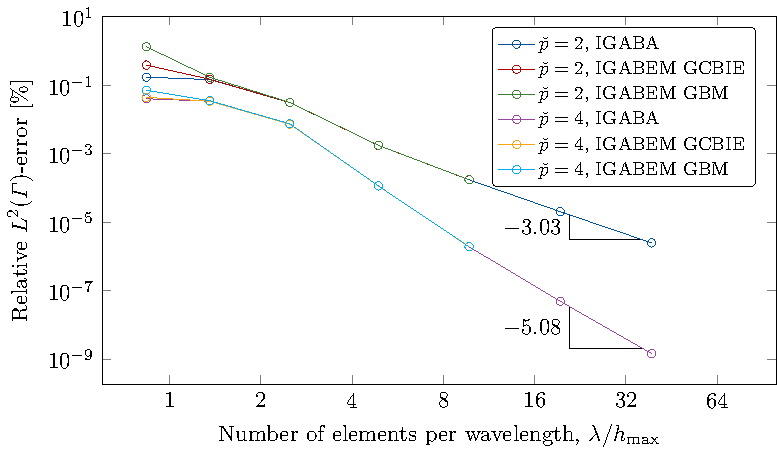
\includegraphics[width=\textwidth]{torus}
	\caption{\textbf{Torus interior acoustic problem}: Convergence analysis at wave number ${k=\SI{2}{m^{-1}}}$.}
	\label{Fig3:torus}
\end{figure}

Results for the same study using collocation formulation are given in \Cref{Fig3:torus_2}. The CCBIE formulation obtains very good results as it approaches the best approximation during refinement. Correct convergence rates are also obtained for the CBM formulation, but with a somewhat higher constant $C_1$ in \Cref{Eq3:aprioriErrorEstimate}.
\begin{figure}
	\centering
	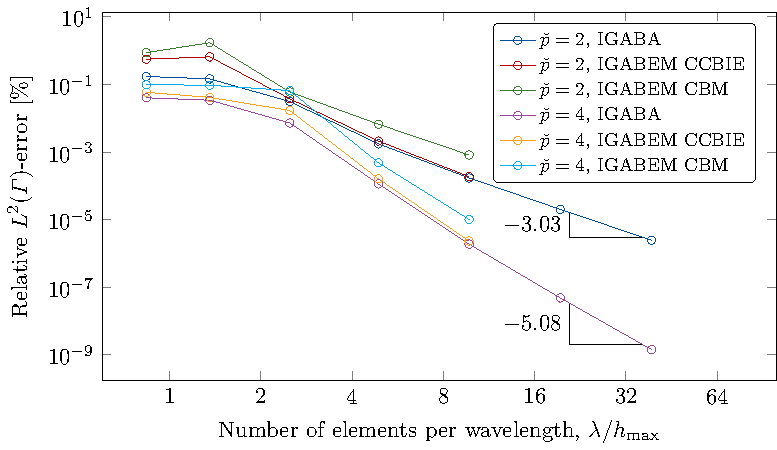
\includegraphics[width=\textwidth]{torus_2}
	\caption{\textbf{Torus interior acoustic problem}: Convergence analysis at wave number ${k=\SI{2}{m^{-1}}}$.}
	\label{Fig3:torus_2}
\end{figure}

In~\cite{Simpson2014aib} Simpson projects the Neumann data onto the same basis used for the solution space. The accuracy for collocation formulations may be increased in some cases using this projection, but for Galerkin formulations projecting the Neumann data yields worse results. Moreover, if $\Gamma$ is $G^0$ sub optimal results are obtained also for the collocation formulations.

\subsection{Manufactured solutions for complex geometries}
In this section we shall consider the method of manufactured solutions (MMS). The idea behind MMS is explained in detail in \cite{Roy2005roc}. 

By construction of the fundamental solution ($\Phi_k(\vec{x},\vec{y})$ in \Cref{Eq3:FreeSpaceGrensFunction}), the function $p(\vec{x}) = \Phi_k(\vec{x},\vec{y})$ is a solution to \Cref{Eq3:HelmholtzEqn,Eq3:HelmholtzEqnNeumannCond,Eq3:sommerfeldCond} whenever $\vec{y}\in\R^3\setminus\overline{\Omega^+}$ and for the Neumann boundary condition $g(\vec{x})=\partial_n\Phi_k(\vec{x},\vec{y})$ on $\Gamma$.  Hence, we have an exact manufactured solution for the exterior Helmholtz problem for arbitrary geometries $\Gamma$ which encloses the point $\vec{y}$. It is emphasized that this solution is non-physical for non-spherical geometries $\Gamma$ (for the sphere, the solution represents a pulsating sphere \cite{Simpson2014aib}). General solutions may be constructed by separation of variables (cf.~\cite[p. 26]{Ihlenburg1998fea})
\begin{equation}
	p(\vec{x}) = \sum_{n=0}^\infty\sum_{m=-n}^n C_{nm} \hankel_n^{(1)}(kR) \legendre_n^{|m|}(\cos\vartheta)\euler^{\imag m\varphi} 
\end{equation}
with
\begin{equation*}
	R = |\vec{x}-\vec{y}|,\quad \vartheta=\arccos\left(\frac{x_3-y_3}{R}\right),\quad\varphi = \operatorname{atan2}(x_2-y_2,x_1-y_1)
\end{equation*}
where $\hankel_n^{(1)}$ is the $n^{\mathrm{th}}$ spherical Hankel function of first kind and $\legendre_n^m$ are the associated Legendre functions. In fact, the solution $p(\vec{x}) = \Phi_k(\vec{x},\vec{y})$ is a special case of this general form with 
\begin{equation}
	C_{nm} = \begin{cases}
		\frac{\imag k}{4\PI} & n = 0,\,\,m=0\\
		0 & \text{otherwise}.
		\end{cases}
\end{equation}
Inspired by the method of fundamental solutions~\cite{Fairweather2003tmo}, we can also use the solution
\begin{equation}\label{Eq3:manuMFS}
	p(\vec{x}) = \sum_{n=1}^N C_n \Phi_k(\vec{x},\vec{y}_n)
\end{equation}
for a set of $N$ source points $\{\vec{y}_n\}_{n=1}^N$. To increase the complexity of the solution, we use $C_n=\cos(n-1)$ in this work.

The complexity of this problem setup does not scale with the complexity of the model as it is independent of $\Gamma$. However, it preserves two important properties of acoustic scattering, namely the radial decay and the oscillatory nature. Thus, this problem setup represents a general way of constructing manufactured solutions that can be utilized to verify the correctness of the implemented code for solving the Helmholtz equation. Moreover, as the boundary condition is the only condition that is altered from the original problem, one can solve the original system of equation with an extra appended column vector on the right-hand side (corresponding to the problem of finding the manufactured solution) with a small computational effort. This gives some control over the correctness of the computed solution to the original problem. Since the fictitious eigenfrequencies are the same for both solutions, one can compute the error for the manufactured solution to give an indication whether the solution is polluted by such a frequency. If this is the case, one should resort to the somewhat more costly Burton--Miller formulation.

Note that from the first limit of \Cref{Eq3:Phi_k_limits}, the far field of \Cref{Eq3:manuMFS} is given by
\begin{equation*}
	p_0(\hat{\vec{x}})=\frac{1}{4\PI}\sum_{n=1}^N C_n \euler^{-\imag k \hat{\vec{x}}\cdot\vec{y}_n}.
\end{equation*}

Whenever $\partial_n p_{\mathrm{tot}}\neq 0$ we must deal with an integral which is weakly singular, and the manufactured solution thus does not give the optimal test for the rigid body scattering problem as the CBIE formulation is free from such integrals in this case.

\subsection{Manufactured solution with a cube}
\begin{figure}
	\centering
	\begin{subfigure}[t]{0.3\textwidth}
		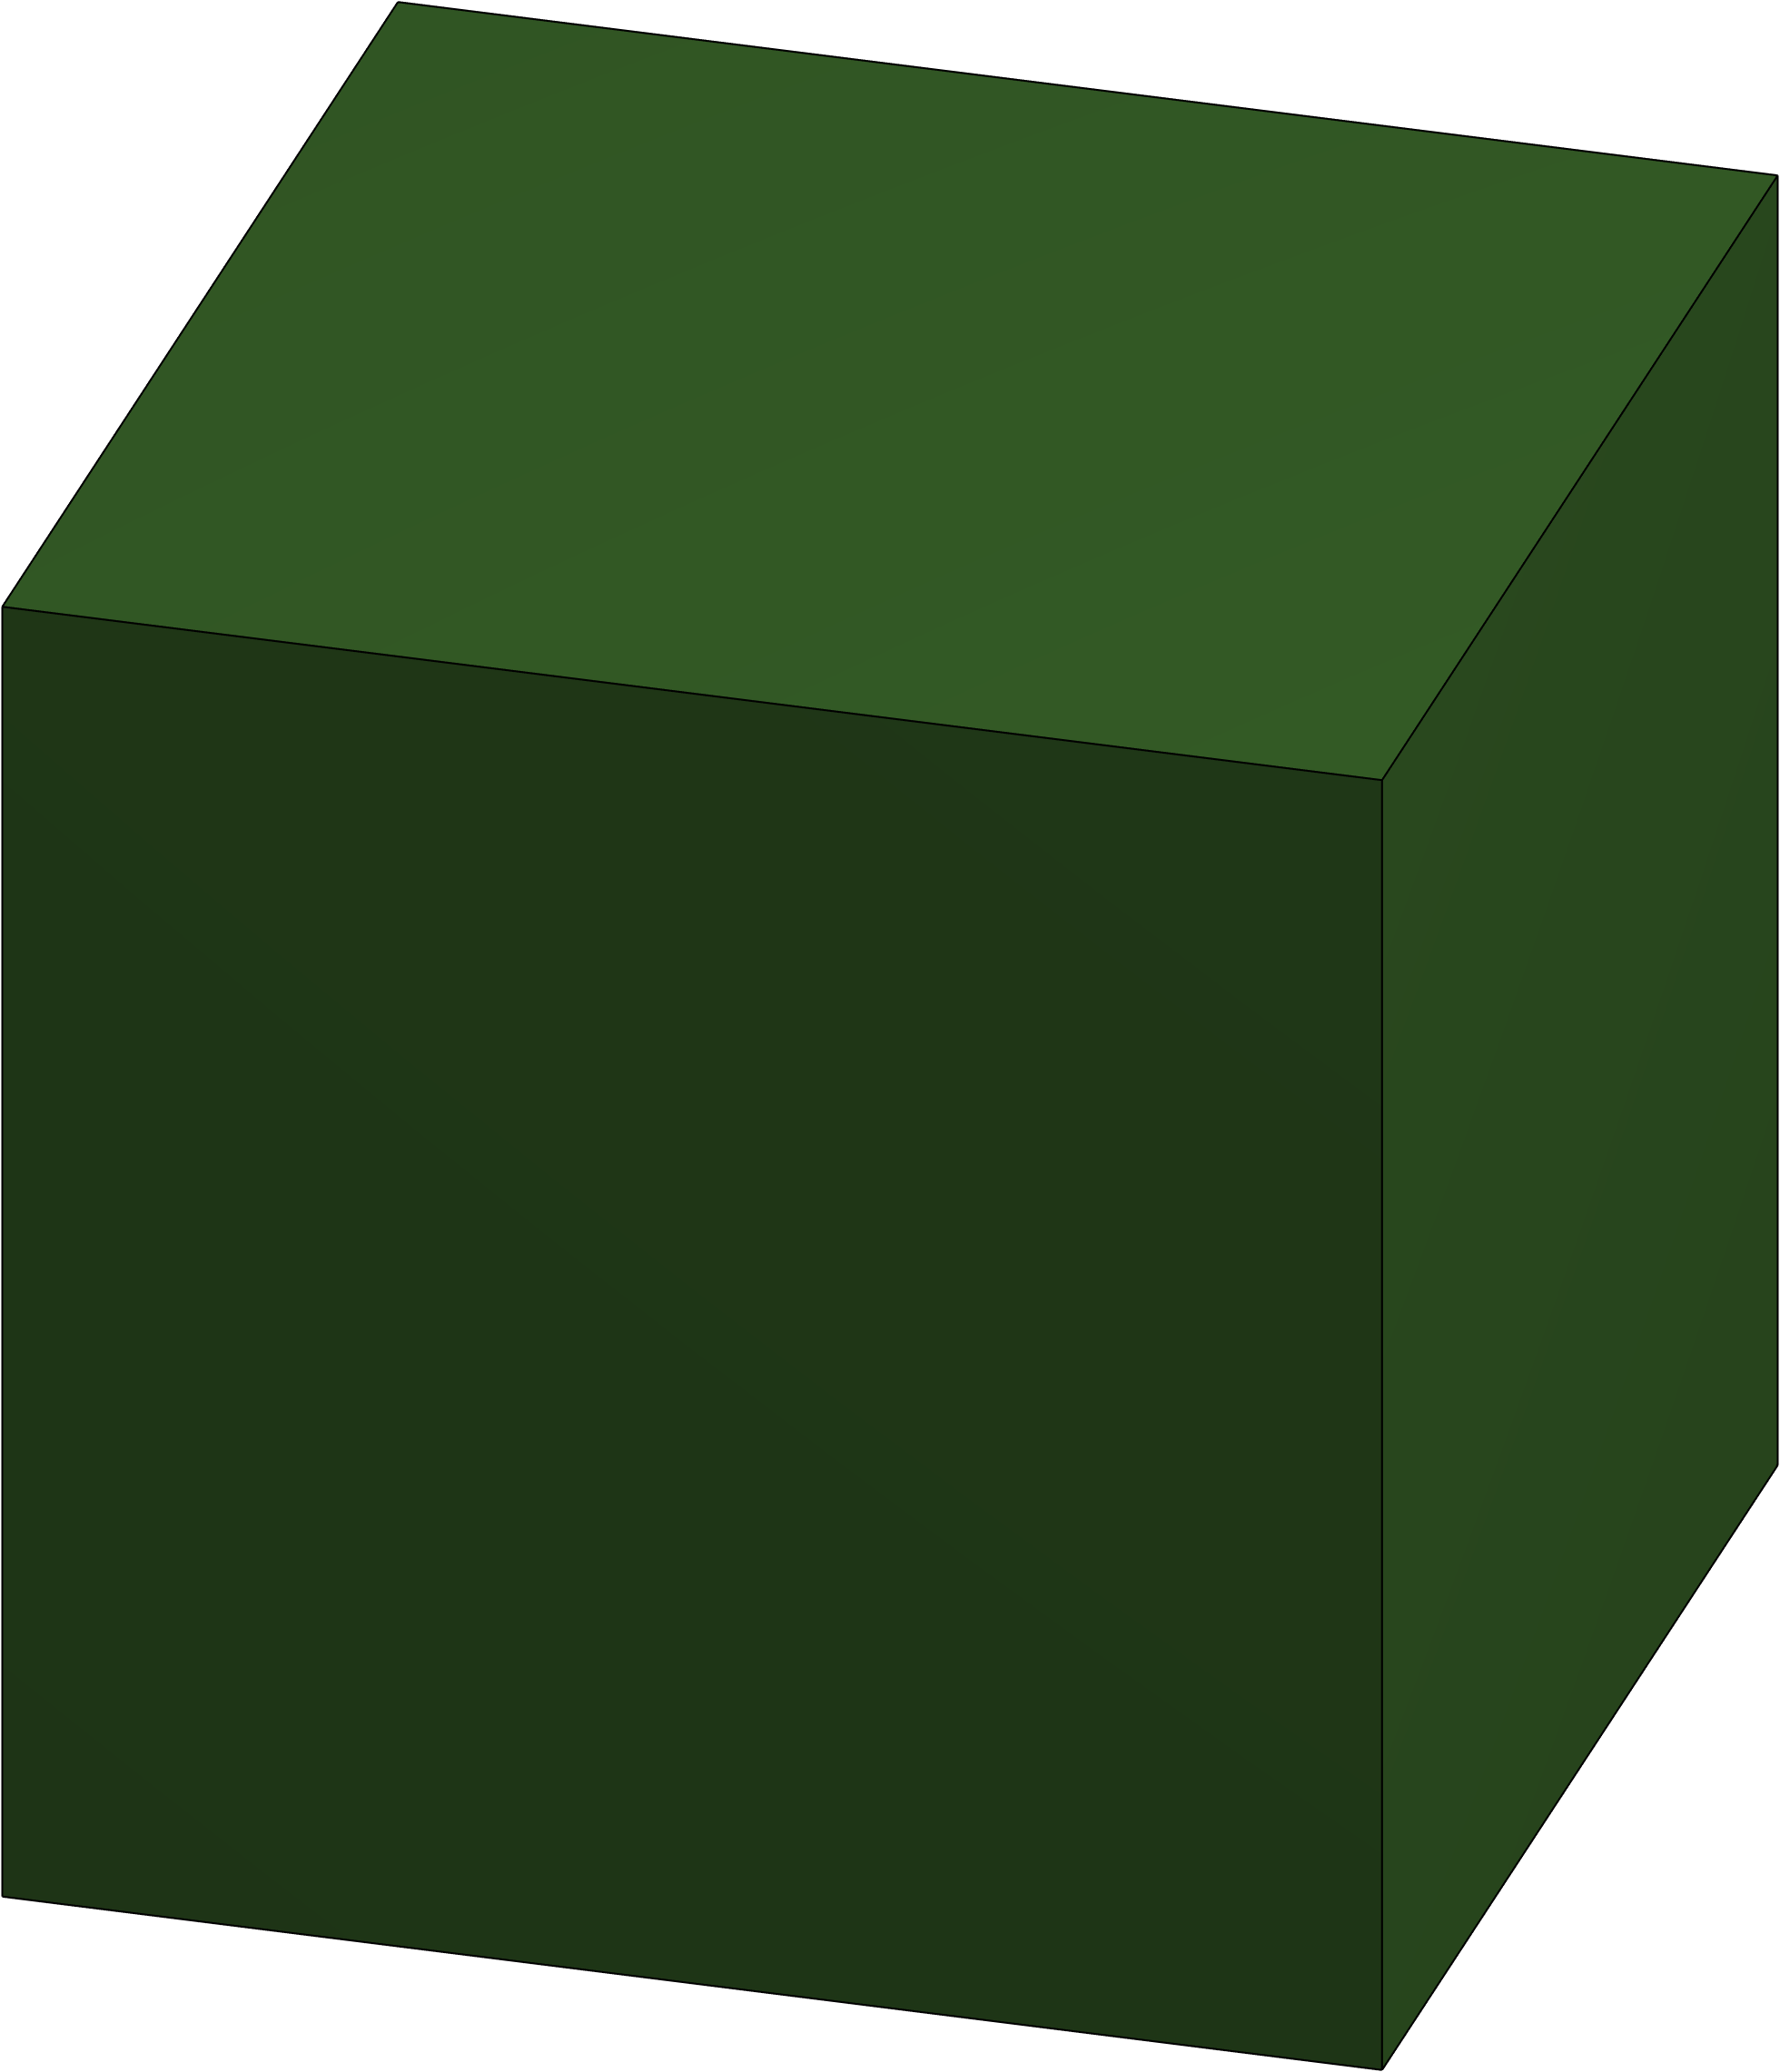
\includegraphics[width=0.9\textwidth]{Cube_mesh1}
		\caption{Mesh 1.}
		\label{Fig3:Cube_mesh1}
	\end{subfigure} 
	~
	\begin{subfigure}[t]{0.3\textwidth}
		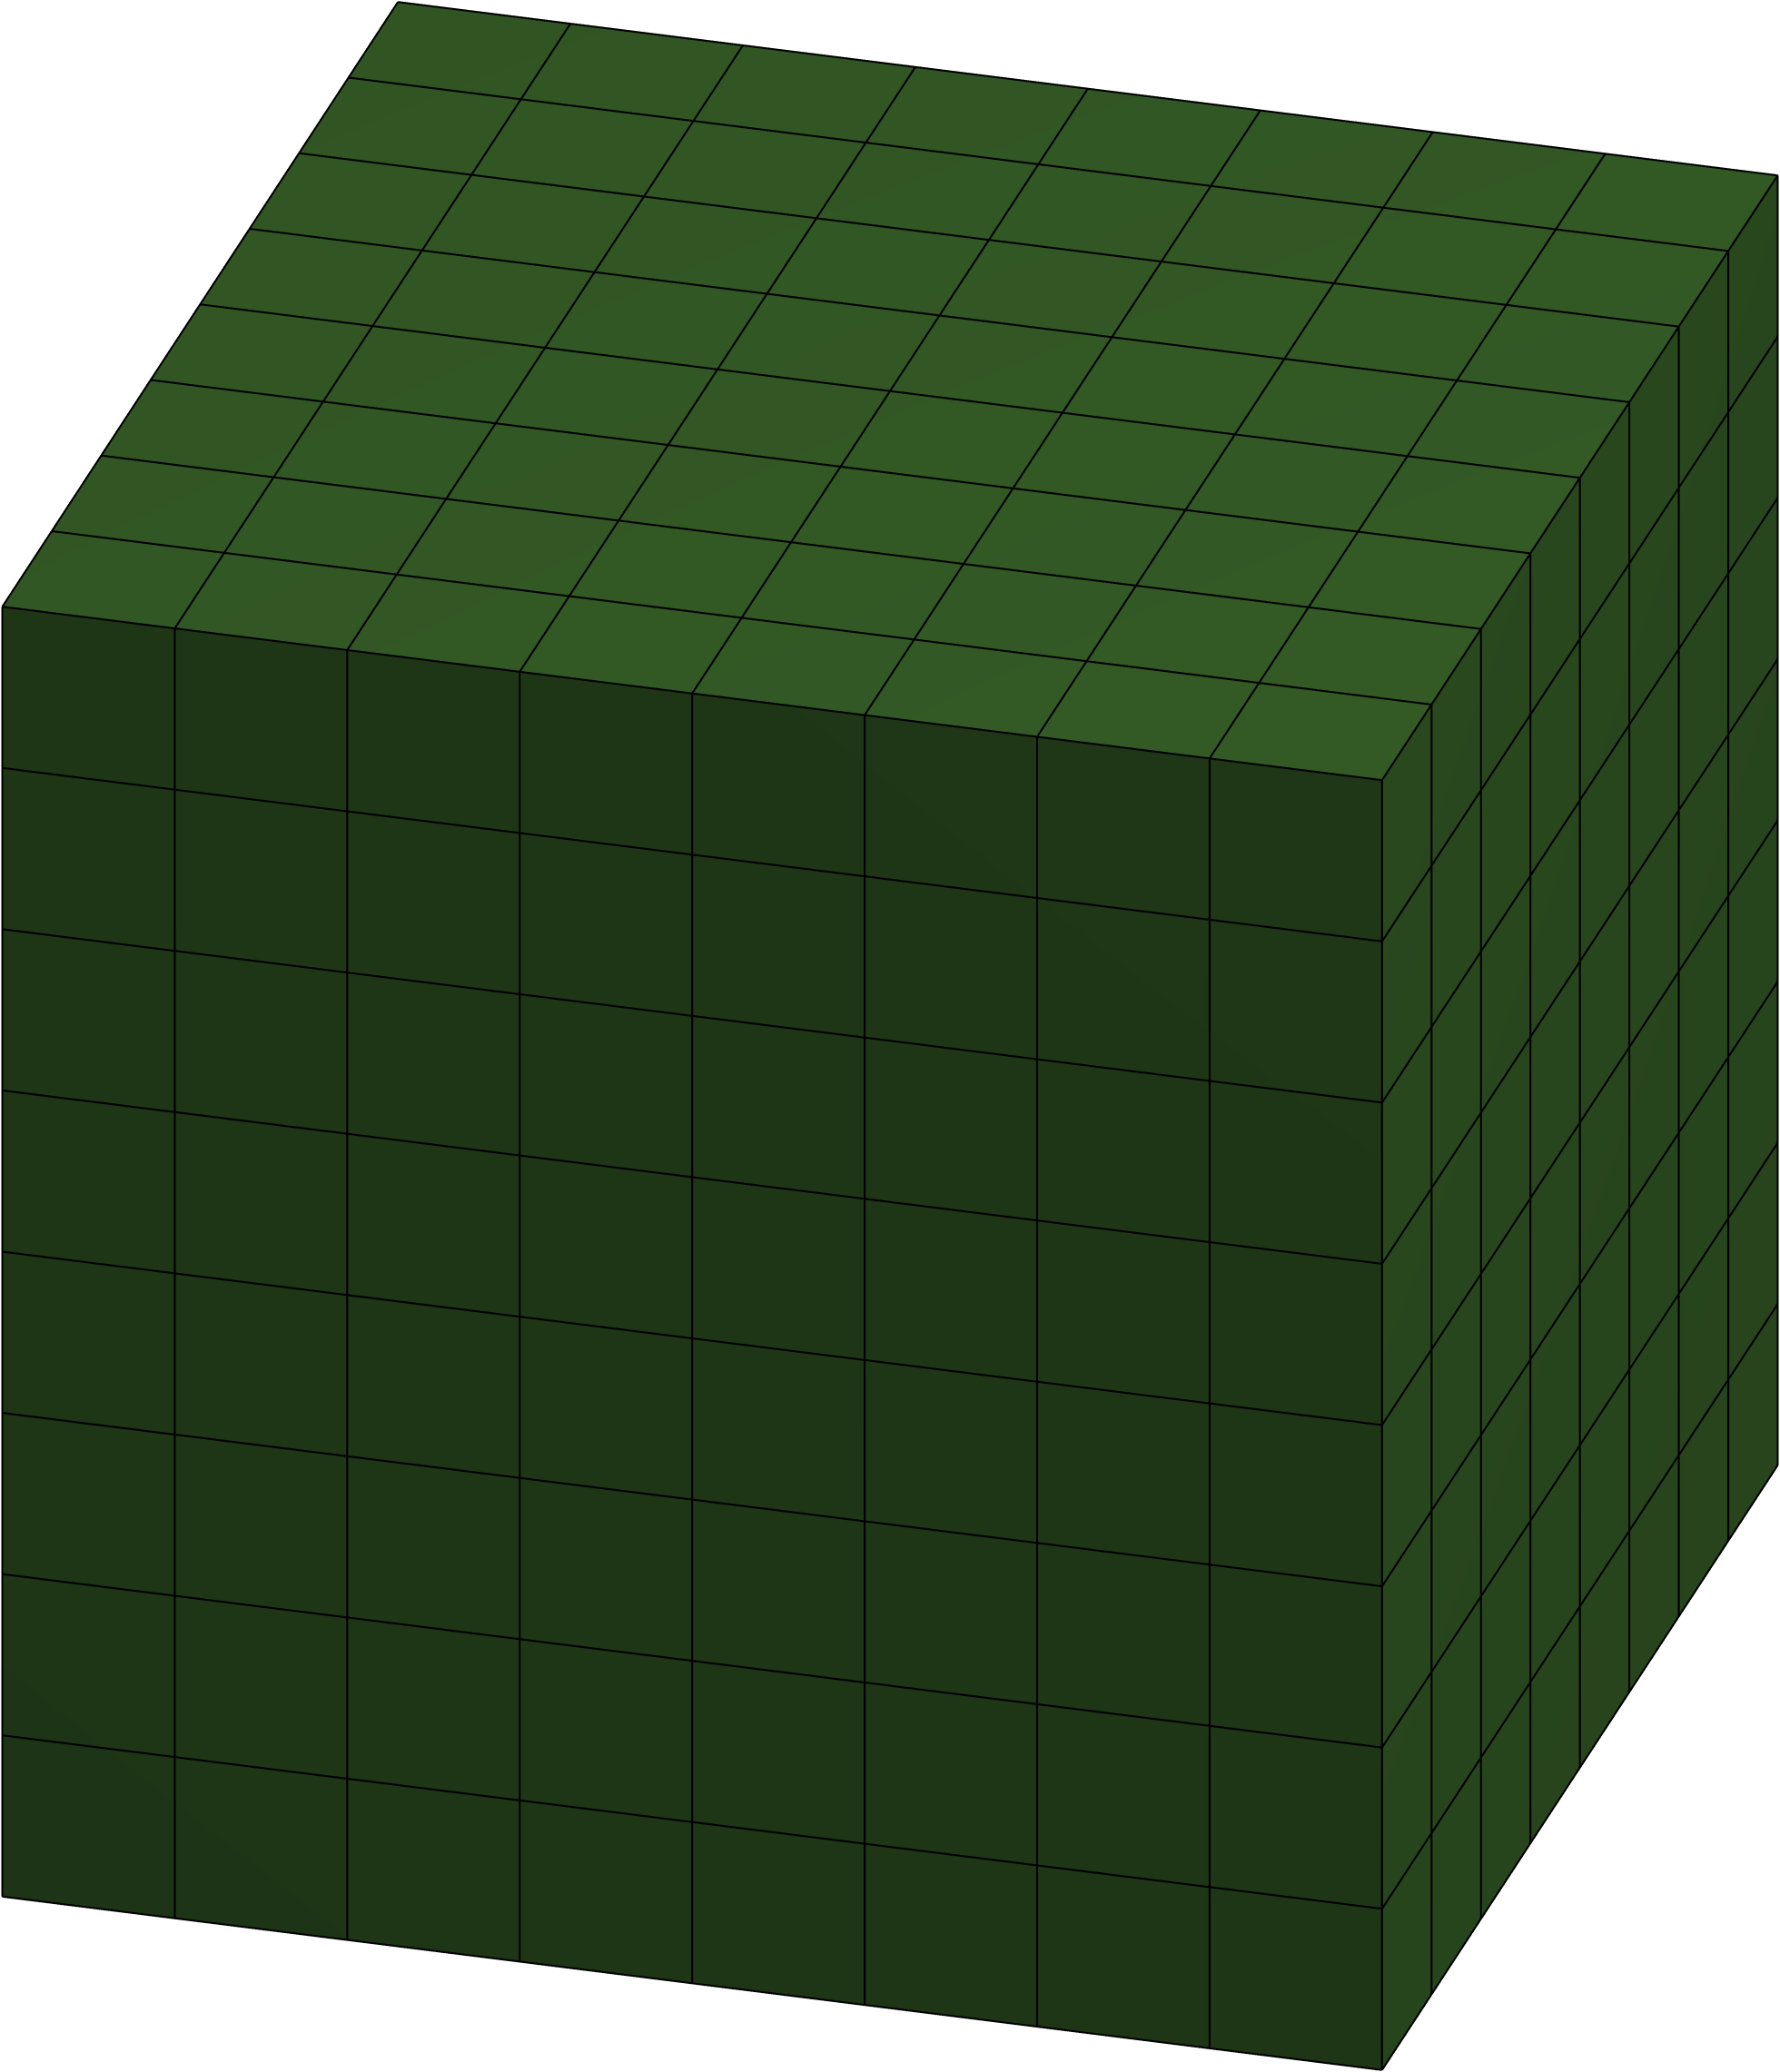
\includegraphics[width=0.9\textwidth]{Cube_mesh4}
		\caption{Mesh 4.}
		\label{Fig3:Cube_mesh4}
	\end{subfigure} 
	\caption{Parametrization of a cube using 6 patches of degree $\check{p}\geq 1$.}
	\label{Fig3:CubeParametrizations}
\end{figure}
Consider a cube of side length $a$ centered at the origin. Its interior Dirichlet problem has eigenfunctions (cf. \cite[p. 52]{Schenck1968iif})
\begin{equation*}
	p(\vec{x}) = \prod_{i=1}^d\sin\frac{n_i\PI (x_i+a/2)}{a},\quad \vec{x}\in\Omega^-
\end{equation*}
and the interior Neumann problem has eigenfunctions
\begin{equation*}
	p(\vec{x}) = \prod_{i=1}^d\cos\frac{n_i\PI (x_i+a/2)}{a},\quad \vec{x}\in\Omega^-
\end{equation*}
where
\begin{equation*}
	\sum_{i=1}^d n_i^2 = \left(\frac{ka}{\PI}\right)^2\quad\text{and}\quad\Omega^-=\left[-\frac{a}{2},\frac{a}{2}\right]^d.
\end{equation*}
The dimensionless eigenfrequencies are thus given by
\begin{equation*}
	ka=\PI\sqrt{\sum_{i=1}^d n_i^2},
\end{equation*}
where $n_i\in\N^*$ for the interior Dirichlet problem and $n_i\in\N$ for the interior Neumann problem. For the exterior problem these eigenfrequencies correspond to the fictitious eigenfrequencies for the CBIE formulation and the HBIE formulation, respectively. The dimensionless fictitious eigenfrequencies below $ka=10$ are then $\PI\sqrt{3}$, $\PI\sqrt{6}$ and $3\PI$ for the CBIE formulation, and $\PI\sqrt{n}$ with $n\in\{0,1,2,3,4,5,6,8,9,10\}$ for the HBIE formulation.

Consider the manufactured solution~\Cref{Eq3:manuMFS} with $N=3^3=27$ source points 
\begin{equation*}
	\vec{y}_n = \frac{a}{4}[c_i, c_j, c_l],\quad n=i+3(j-1)+3^2(l-1),\quad i,j,l=1,2,3
\end{equation*}
where $c_1=-1$, $c_2=0$ and $c_3=1$. In~\Cref{Fig3:Cube_P_sweep} we again show a frequency sweep to illustrate the instability around the fictitious eigenfrequencies of the CBIE and HBIE formulations.
\begin{figure}
	\centering
	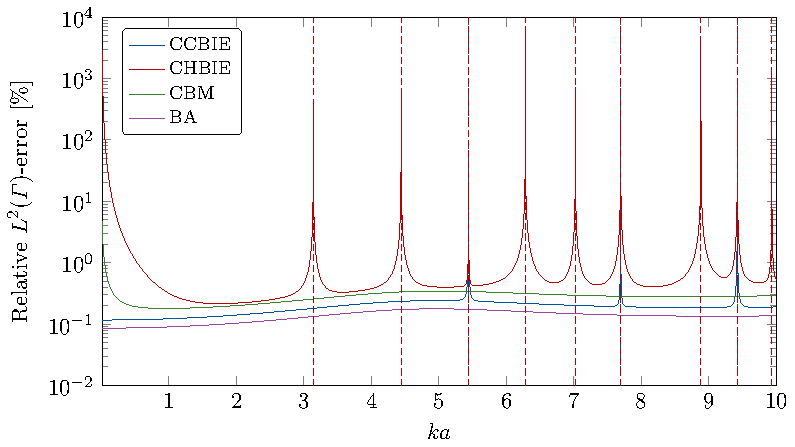
\includegraphics[width=\textwidth]{Cube_P_sweep}
	\caption{\textbf{Manufactured solution with a cube}: The plots show the instabilities around eigenfrequencies of the corresponding interior Dirichlet problem. All computations are done using the parametrization in \Cref{Fig3:Cube_mesh1} refined uniformly three times with NURBS degree 4 (resulting in 384 elements and 728 degrees of freedom) as highlighted in \Cref{Fig3:Cube_mesh4}.}
	\label{Fig3:Cube_P_sweep}
\end{figure}
From \Cref{Fig3:Cube_P1}, the sharpness of the a priori error estimate in \Cref{Eq3:aprioriErrorEstimate} is again demonstrated. Remarkably, the $G^0$ continuity of the cube poses no problems for the Galerkin Burton--Miller formulation using $\check{p}\geq 2$, despite the problematic mathematical nature of the formulations with basis functions that are $C^0$ continuous~\cite{Liu1999anf}. Poor results are obtained for the BM formulation using $\check{p}=1$ for both collocation and Galerkin formulation. This is in stark contrast to the CBIE which performs optimally for $\check{p}=1$ in both cases. The CCBIE obtains good results in all cases and outperforms the CBM formulation.
\begin{figure}
	\centering
	\begin{subfigure}[t]{\textwidth}
		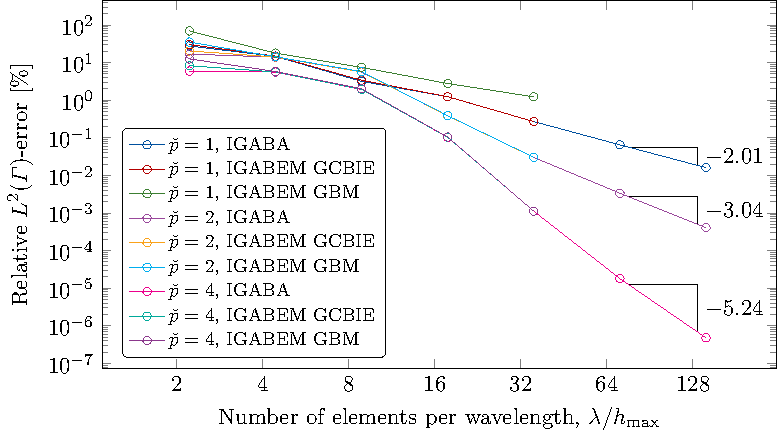
\includegraphics[width=\textwidth]{cube_P}
		\caption{Galerkin formulations}
		\label{Fig3:Cube_P1}
	\end{subfigure} 
	\par\bigskip
	\par\bigskip
	\begin{subfigure}[t]{\textwidth}
		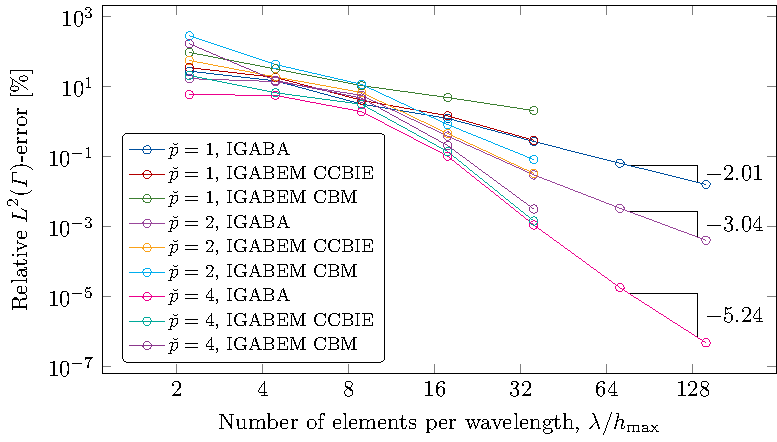
\includegraphics[width=\textwidth]{cube_P_2}
		\caption{Collocation formulations}
		\label{Fig3:Cube_P2}
	\end{subfigure} 
	\caption{\textbf{Manufactured solution with a cube}: Convergence analysis at $k=\SI{2}{m^{-1}}$.}
	\label{Fig3:Cube_P}
\end{figure}

\subsection{Manufactured solution with the BeTSSi submarine}
\label{Subsec3:manufactured}
\begin{figure}
	\centering
	\begin{subfigure}[t]{\textwidth}
		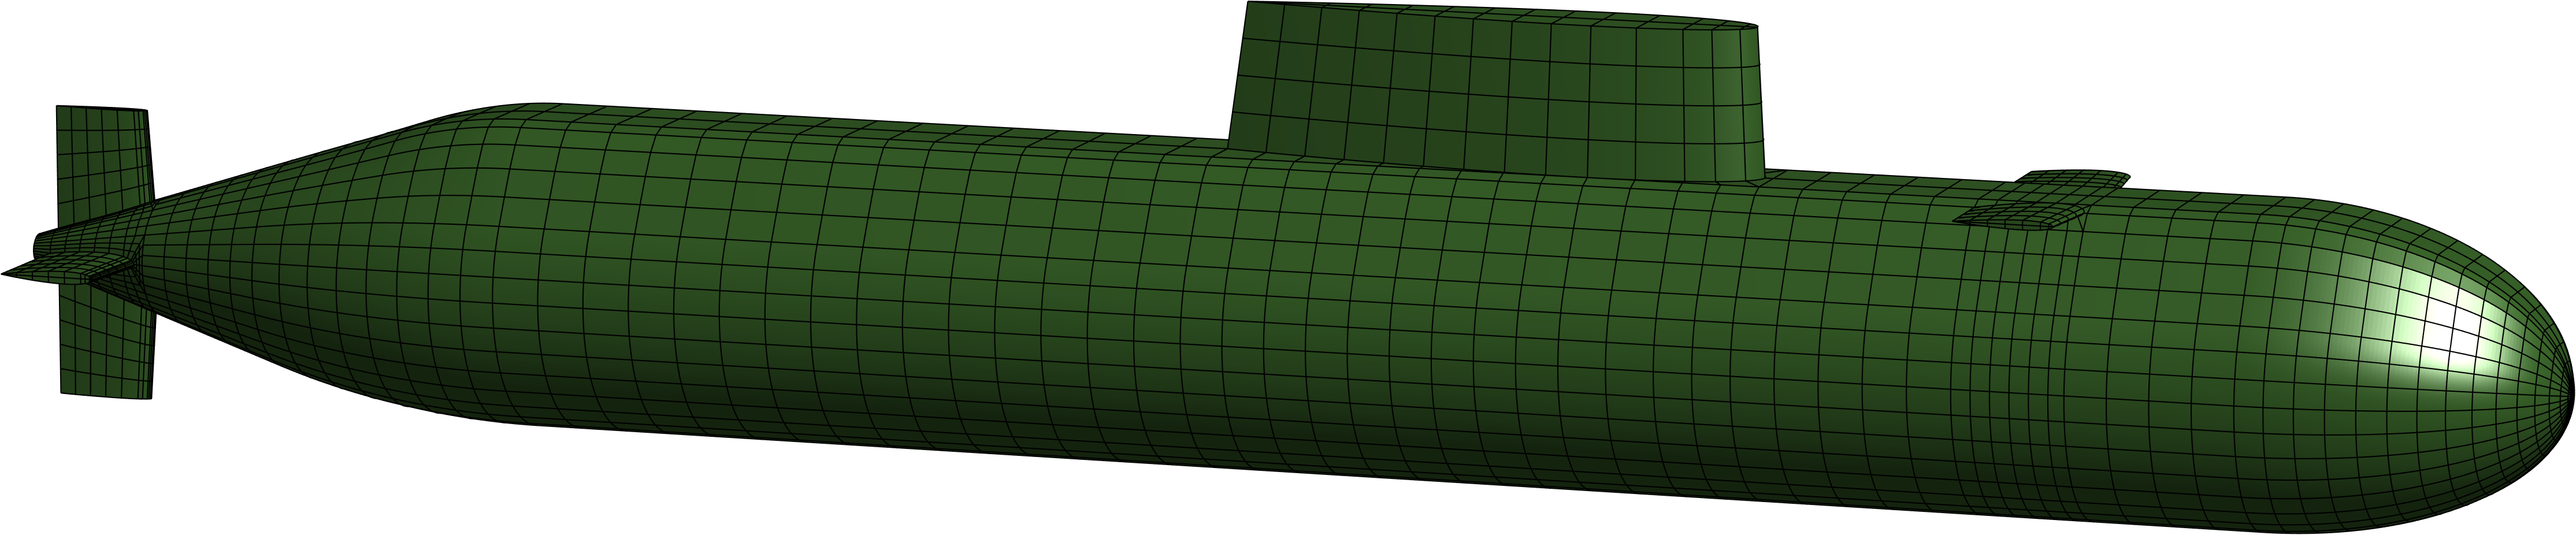
\includegraphics[width=\textwidth]{mesh1}
		\caption{${\cal M}_{1,6,5}^{\textsc{igabem}}$ - 3718 elements}
	\end{subfigure} 
	\par\bigskip
	\par\bigskip
	\begin{subfigure}[t]{\textwidth}
		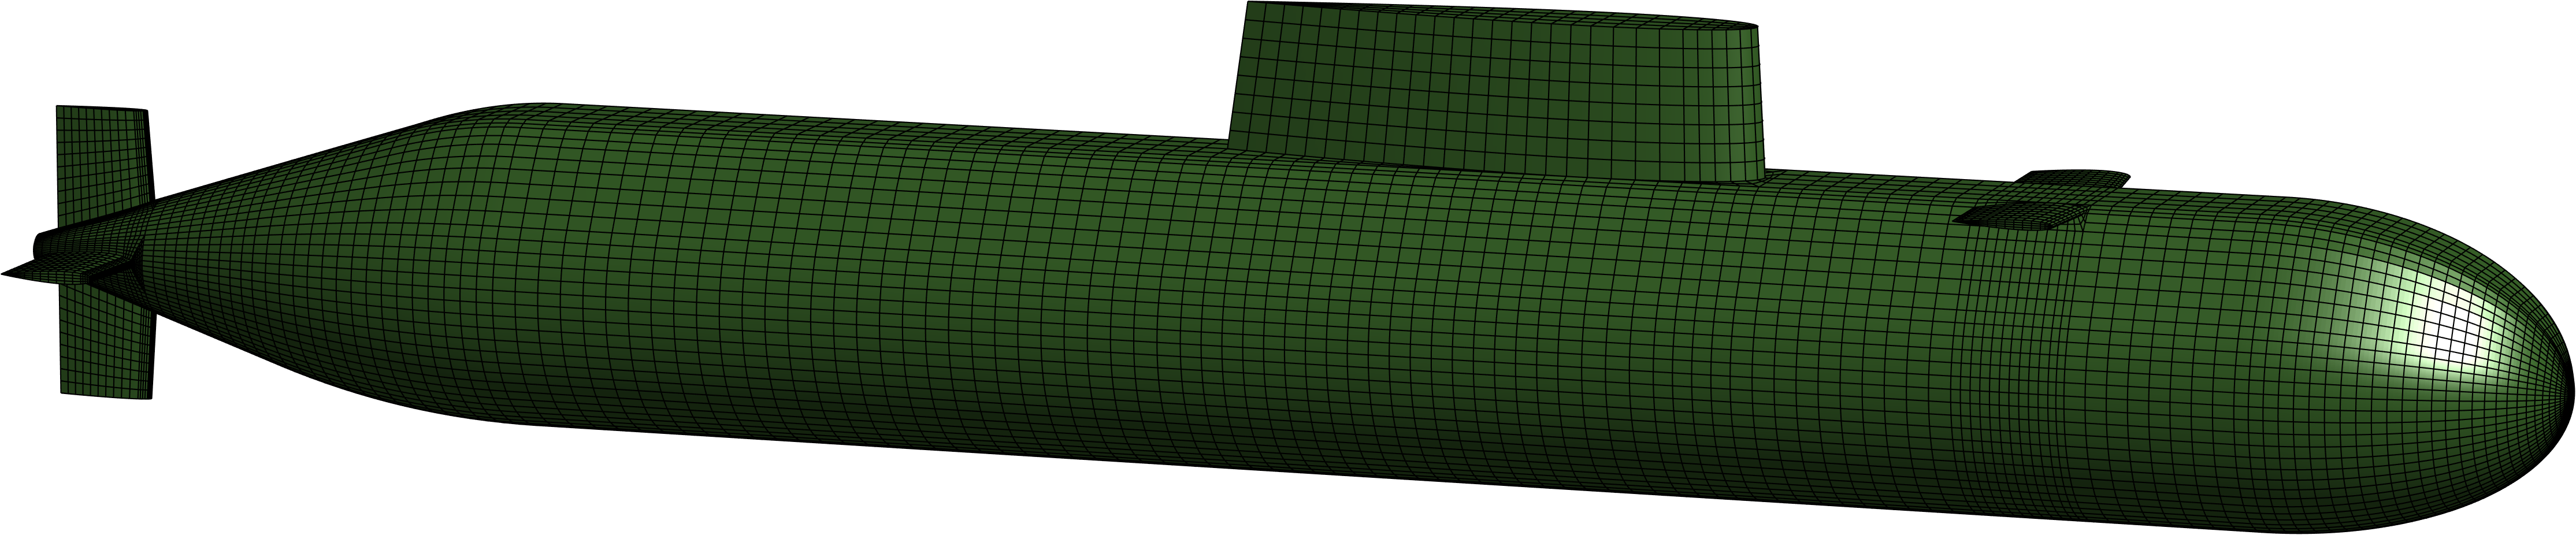
\includegraphics[width=\textwidth]{mesh2}
		\caption{${\cal M}_{2,6,5}^{\textsc{igabem}}$ - 14872 elements}
	\end{subfigure} 
	\par\bigskip
	\par\bigskip
	\begin{subfigure}[t]{\textwidth}
		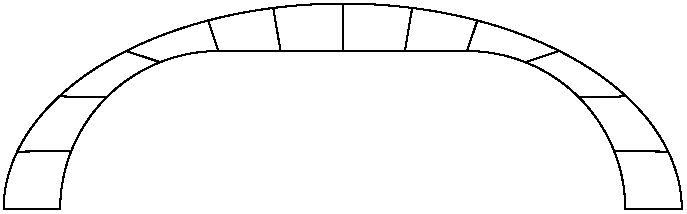
\includegraphics[width=\textwidth]{mesh3}
		\caption{${\cal M}_{3,6,5}^{\textsc{igabem}}$ - 59488 elements}
	\end{subfigure} 
	\caption{\textbf{The BeTSSi submarine}: Computational IGA meshes for $\Gamma_{\check{p}}$ with $\check{p}=6$.}
	\label{Fig3:BeTSSimeshes}
\end{figure}
Consider now the BeTSSi submarine described in \Cref{Sec3:BeTSSi_description}. The BeTSSi meshes considered in this work are denoted by ${\cal M}_{m,\check{p},\check{k}}^{\textsc{igabem}}$, where $m$ is the mesh number, and are illustrated in \Cref{Fig3:BeTSSimeshes} where $m=1$ is the coarsest mesh, and $m=2$ and $m=3$ are uniformly refined meshes iterated on the coarsest mesh. Again, $\check{p}$ denotes the polynomial order and $\check{k}$ the continuity.

Consider the manufactured solution~\Cref{Eq3:manuMFS} on the BeTSSi submarine with $N=16$ and where 16 source points are uniformly placed at the $x$-axis starting at $x=b$ and ending at $x=-L-2b$ (parameters taken from \Cref{Tab3:BeTSSiParameters}). The analytic real part of the pressure, $\Re{p}$, is visualized on the surface of the scatterer in~\Cref{Fig3:BCA_P_analytic}. 
\begin{figure}
	\centering
	\begin{subfigure}[t]{\textwidth}
		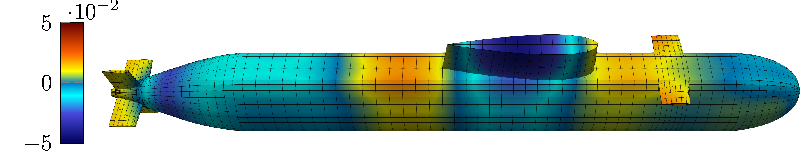
\includegraphics[width=\textwidth]{BCA_P_analyticF100}
		\caption{$f=\SI{100}{Hz}$}
	\end{subfigure} 
	\par\bigskip
	\begin{subfigure}[t]{\textwidth}
		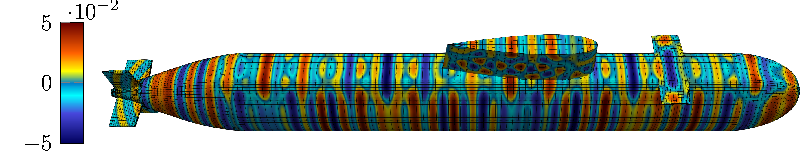
\includegraphics[width=\textwidth]{BCA_P_analyticF1000}
		\caption{$f=\SI{1000}{Hz}$}
	\end{subfigure} 
	\caption{\textbf{Manufactured solution with the BeTSSi submarine}: Analytic manufactured solution. Mesh 1 and mesh 2 are added to visualize elements to wavelength ratio for $\SI{100}{Hz}$ and $\SI{1000}{Hz}$, respectively.}
	\label{Fig3:BCA_P_analytic}
\end{figure}
A simulation at $f=\SI{100}{Hz}$ on mesh ${\cal M}_{1,2,1}^{\textsc{igabem}}$ yields the error plots in~\Cref{Fig3:BCA_P_p2M1f100}, which show good agreement between the best approximation and the BEM simulation. For more refined meshes in \Cref{Fig3:BCA_P_p5M1f100,Fig3:BCA_P_p2M2f100,Fig3:BCA_P_p5M2f100} (especially \Cref{Fig3:BCA_P_p5M2f100}) the numerical quadrature around the source points is too inaccurate. At this level of numerical accuracy, one quickly runs into issues due to round-off errors. The non-Lipschitz domains do not in and of itself pose any analysis suitable issues as described in~\Cref{Sec3:BeTSSi_approximation}, so the effect seen here is due to the numerical integration in the boundary element method. At $f=\SI{1000}{Hz}$ it is clear from \Cref{Fig3:BCA_P_p5M2f1000} that the IGABEM CCBIE simulation is polluted from a fictitious eigenfrequency. The remedy for this is to use the CBM formulation which obtains results with maximal error roughly twice the size of the best approximation. The meshes for the BeTSSi submarine in~\Cref{Fig3:BeTSSimeshes} might give the impression of evenly distributed control points in some areas, in particular the area behind the sail ($-L<x<x_{\mathrm{s}}-l_{\mathrm{ls}}$). In this case there are additional knot insertions around the submarine to obtain the $C^0$ lines, which results in ``bands'' of slightly larger errors along the submarine. This effect will be larger for higher polynomial orders, particularly for mesh ${\cal M}_{2,5,4}^{\textsc{igabem}}$ in~\Cref{Fig3:BCA_P_p5M2f1000_BA}.
\begin{figure}
	\centering
	\begin{subfigure}[t]{\textwidth}
		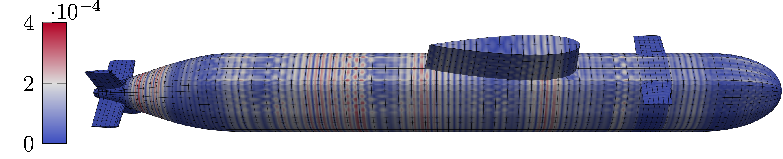
\includegraphics[width=\textwidth]{BCA_P_BAp2M1f100}
		\caption{IGABA: $\displaystyle \max_{\vec{x}\in\Gamma_2}\frac{|p-p_h|}{|p|} = \num{3.8e-4}$}
	\end{subfigure} 
	\par\bigskip
	\begin{subfigure}[t]{\textwidth}
		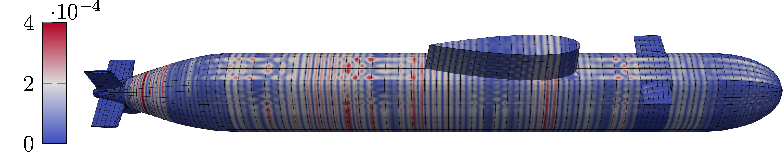
\includegraphics[width=\textwidth]{BCA_P_BEMp2M1f100}
		\caption{IGABEM CCBIE: $\displaystyle \max_{\vec{x}\in\Gamma_2}\frac{|p-p_h|}{|p|} = \num{4.0e-4}$}
	\end{subfigure} 
	\caption{\textbf{Manufactured solution with the BeTSSi submarine}: Relative error on the surface of the scatterer at $f=\SI{100}{Hz}$ on the mesh ${\cal M}_{1,2,1}^{\textsc{igabem}}$.}
	\label{Fig3:BCA_P_p2M1f100}
\end{figure}


\begin{figure}
	\centering
	\begin{subfigure}[t]{\textwidth}
		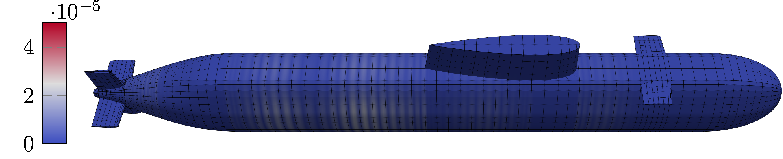
\includegraphics[width=\textwidth]{BCA_P_BAp5M1f100}
		\caption{IGABA: $\displaystyle \max_{\vec{x}\in\Gamma_5}\frac{|p-p_h|}{|p|} = \num{2.1e-5}$}
	\end{subfigure} 
	\par\bigskip
	\begin{subfigure}[t]{\textwidth}
		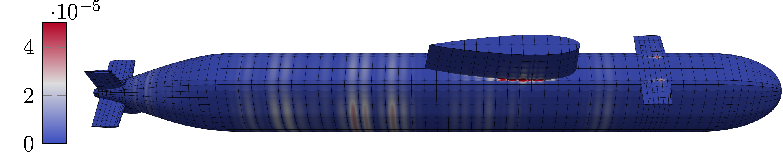
\includegraphics[width=\textwidth]{BCA_P_BEMp5M1f100}
		\caption{IGABEM CCBIE: $\displaystyle \max_{\vec{x}\in\Gamma_5}\frac{|p-p_h|}{|p|} = \num{4.4e-4}$}
	\end{subfigure} 
	\caption{\textbf{Manufactured solution with the BeTSSi submarine}: Relative error on the surface of the scatterer at $f=\SI{100}{Hz}$ on the mesh ${\cal M}_{1,5,4}^{\textsc{igabem}}$.}
	\label{Fig3:BCA_P_p5M1f100}
\end{figure}


\begin{figure}
	\centering
	\begin{subfigure}[t]{\textwidth}
		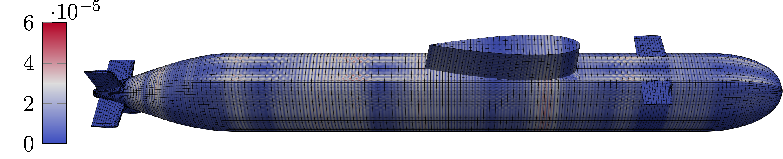
\includegraphics[width=\textwidth]{BCA_P_BAp2M2f100}
		\caption{IGABA: $\displaystyle \max_{\vec{x}\in\Gamma_2}\frac{|p-p_h|}{|p|} = \num{6.1e-5}$}
	\end{subfigure} 
	\par\bigskip
	\begin{subfigure}[t]{\textwidth}
		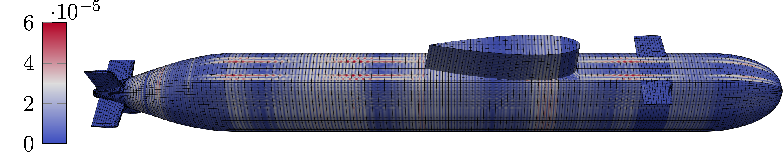
\includegraphics[width=\textwidth]{BCA_P_BEMp2M2f100}
		\caption{IGABEM CCBIE: $\displaystyle \max_{\vec{x}\in\Gamma_2}\frac{|p-p_h|}{|p|} = \num{2.3e-4}$}
	\end{subfigure} 
	\caption{\textbf{Manufactured solution with the BeTSSi submarine}: Relative error on the surface of the scatterer at $f=\SI{100}{Hz}$ on the mesh ${\cal M}_{2,2,1}^{\textsc{igabem}}$.}
	\label{Fig3:BCA_P_p2M2f100}
\end{figure}


\begin{figure}
	\centering
	\begin{subfigure}[t]{\textwidth}
		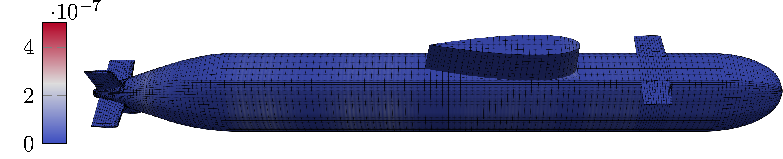
\includegraphics[width=\textwidth]{BCA_P_BAp5M2f100}
		\caption{IGABA: $\displaystyle \max_{\vec{x}\in\Gamma_5}\frac{|p-p_h|}{|p|} = \num{1.7e-7}$}
	\end{subfigure} 
	\par\bigskip
	\begin{subfigure}[t]{\textwidth}
		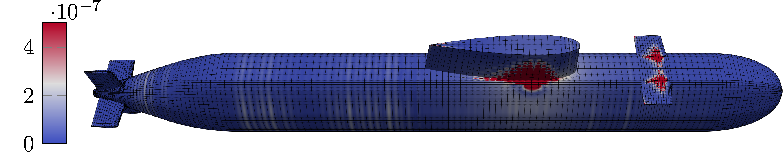
\includegraphics[width=\textwidth]{BCA_P_BEMp5M2f100}
		\caption{IGABEM CCBIE: $\displaystyle \max_{\vec{x}\in\Gamma_5}\frac{|p-p_h|}{|p|} = \num{7.8e-4}$}
	\end{subfigure} 
	\caption{\textbf{Manufactured solution with the BeTSSi submarine}: Relative error on the surface of the scatterer at $f=\SI{100}{Hz}$ on the mesh ${\cal M}_{2,5,4}^{\textsc{igabem}}$.}
	\label{Fig3:BCA_P_p5M2f100}
\end{figure}


\begin{figure}
	\centering
	\begin{subfigure}[t]{\textwidth}
		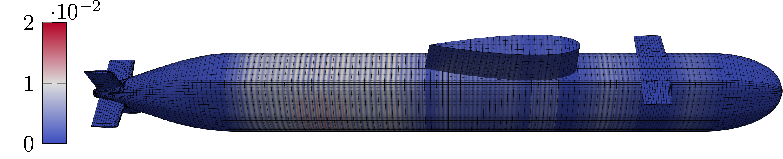
\includegraphics[width=\textwidth]{BCA_P_BAp5M2f1000}
		\caption{IGABA: $\displaystyle \max_{\vec{x}\in\Gamma_5}\frac{|p-p_h|}{|p|} = 0.014$}
		\label{Fig3:BCA_P_p5M2f1000_BA}
	\end{subfigure} 
	\par\bigskip
	\begin{subfigure}[t]{\textwidth}
		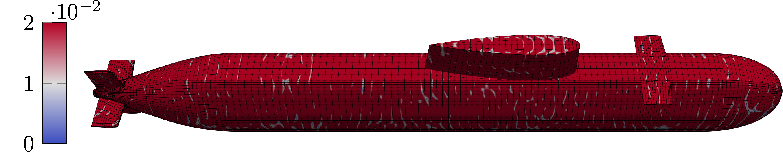
\includegraphics[width=\textwidth]{BCA_P_BEMp5M2f1000}
		\caption{IGABEM CCBIE: $\displaystyle \max_{\vec{x}\in\Gamma_5}\frac{|p-p_h|}{|p|} = 0.40$}
	\end{subfigure} 
	\par\bigskip
	\begin{subfigure}[t]{\textwidth}
		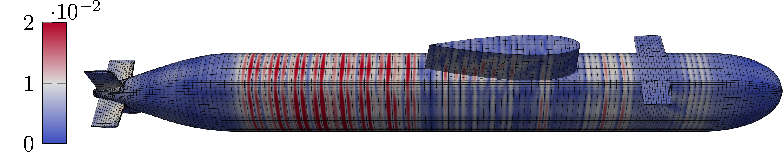
\includegraphics[width=\textwidth]{BCA_P_BEMp5M2f1000_CBM}
		\caption{IGABEM CBM: $\displaystyle \max_{\vec{x}\in\Gamma_5}\frac{|p-p_h|}{|p|} = 0.030$}
	\end{subfigure} 
	\caption{\textbf{Manufactured solution with the BeTSSi submarine}: Relative error on the surface of the scatterer at $f=\SI{1000}{Hz}$ on the mesh ${\cal M}_{2,5,4}^{\textsc{igabem}}$.}
	\label{Fig3:BCA_P_p5M2f1000}
\end{figure}

To assess the parameter $s_1$ in~\Cref{Eq3:numberOfSubElements}, a low frequency of $\SI{100}{Hz}$ is now considered. In \Cref{Fig3:BCA_P_qp} we illustrate the effect of different choices of the parameter $s_1$ for the more complex geometry of the BeTSSi submarine. Again, the optimal choice for $s_1$ is polynomial dependent. Moreover, even the regularized formulations CRCBIE1 and CRCBIE3 must have $s_1>0$ contrary to what was proposed in~\cite{Sun2015bri} (stating that the singular free integrals ``can be evaluated by any convenient integration quadrature''). Whenever care is not taken for the numerical quadrature, incorrect conclusions may arise. This example illustrates the power of the manufactured solution as it enables computation of the best approximation such that the numerical integration may be controlled.
\begin{figure}
	\centering    
	\begin{subfigure}[t]{0.49\textwidth}
		\centering
		\includegraphics{BCA_P_qp_1}
		\caption{$\check{p} = 2$}
	\end{subfigure}%
	\hspace*{0.02\textwidth}%
	\begin{subfigure}[t]{0.49\textwidth}
		\centering
		\includegraphics{BCA_P_qp_2}
		\caption{$\check{p} = 5$}
	\end{subfigure}
	\caption{\textbf{Manufactured solution with the BeTSSi submarine}: Surface error as a function of the parameter $s_1$, on the mesh ${\cal M}_{1,\check{p},\check{p}-1}^{\textsc{igabem}}$.}
	\label{Fig3:BCA_P_qp}
\end{figure}

\subsection{Rigid scattering on the BeTSSi submarine}
Consider now a plane wave scattered by a rigid BeTSSi submarine. Throughout this section (motivated by the previous section) we use the CCBIE formulation at $f=\SI{100}{Hz}$ and the CBM formulation at $f=\SI{1000}{Hz}$. To verify our simulations, we compare with corresponding simulations done in \COMSOL, with mesh and parameters as illustrated and described in~\Cref{Fig3:COMSOL}. Comparisons are also made with simulations done by WTD 71\footnote{Wehrtechnische Dienststelle f\"{u}r Schiffe und Marinewaffen, Maritime Technologie und Forschung.}.
\begin{figure}
	\centering
	\includegraphics[width=\textwidth]{comsol}
	\caption{\textbf{Rigid scattering on the BeTSSi submarine}: Mesh used in \COMSOL simulations. The mesh consists of \num{27614929} second order finite elements including the elements in the PML (resulting in \num{43431671} degrees of freedom). This corresponds to 80 and 8 elements per wavelength for $\SI{100}{Hz}$ and $\SI{1000}{Hz}$, respectively.  The PML domain consists of a cylinder with two spherical end caps and are discretized by 10 layers of prismatic elements. The domain inside this PML is discretized with tetrahedral elements. The distance between the PML and the scatterer at the $x$-axis is $t_{\mathrm{a}}=\SI{1}{m}$ at both ends. The thickness of the PML is the same as the maximal tetrahedral diameter $h_{\mathrm{max}}=\SI{0.1875}{m}$. The PML cylinder starts at $x=-L-g_2-g_3+a$ and ends at $x=0$. The radius of the PML cylinder and the PML spherical end caps are $r_{\mathrm{a}} = a+t_{\mathrm{a}}$. The PML uses a polynomial coordinate stretching type with scaling factor and scaling curvature equal to 1. The simulations use \COMSOL version 5.4 with the acoustics module (to enable the PML method) and the design module (to import the CAD model).}
	\label{Fig3:COMSOL}
\end{figure}
The polar plot in \Cref{Eq3:polar_BI} illustrates bistatic scattering where the incident wave is fixed, and the observation points for the far field computations sweep the aspect angles. A very good match is obtained, although some discrepancies are observed around the aft angles (around $\alpha=\ang{180}$). One can argue that the logarithmic scale of the target strength (TS) yields a somewhat misguided conception of the numerical error in the pressure. The pressure at these angles is very low such that the global relative error in the pressure is not as bad as the plot may suggest.
\begin{figure}
	\centering
	\includegraphics[width=\textwidth]{PolarPlot_6}
	\caption{\textbf{Rigid scattering on the BeTSSi submarine}: Polar plot of the bistatic target strength ($\TS$) plotted against the azimuth angle $\varphi$ at $f=\SI{1000}{Hz}$. Direction of incident wave, $p_{\mathrm{inc}}$ is given by \Cref{Eq3:d_s} with $\alpha_{\mathrm{s}}=\ang{240}$ and $\beta_{\mathrm{s}}=\ang{0}$. The IGA mesh here used is ${\cal M}_{3,5,4}^{\textsc{igabem}}$. The \COMSOL simulation used \num{3.8} hours on mesh ${\cal M}_{4,2,0}^{\textsc{comsol}}$. The WTD 71 simulation was made using a direct BEM collocation method with the Burton--Miller formulation on mesh ${\cal M}_{5}^{\textsc{wtd}}$ described in \Cref{Sec3:BeTSSi_triangulation} with constant basis functions over each element.}
	\label{Eq3:polar_BI}
\end{figure}
In \Cref{Fig3:xy_BI_100} and \Cref{Fig3:xy_BI_1000} the corresponding $xy$-plots are given at $\SI{100}{Hz}$ and $\SI{1000}{Hz}$, respectively.
\begin{figure}
	\centering
	\begin{subfigure}[t]{\textwidth}
		\includegraphics[width=\textwidth]{BCA_farField_1}
		\caption{$f=\SI{100}{Hz}$}
		\label{Fig3:xy_BI_100}
	\end{subfigure} 
	\par\bigskip
	\par\bigskip
	\begin{subfigure}[t]{\textwidth}
		\includegraphics[width=\textwidth]{BCA_farField_2}
		\caption{$f=\SI{1000}{Hz}$}
		\label{Fig3:xy_BI_1000}
	\end{subfigure} 
	\caption{\textbf{Rigid scattering on the BeTSSi submarine}: The bistatic target strength ($\TS$) plotted against the azimuth angle $\varphi$.}
\end{figure}
In~\Cref{Fig3:xy_BI_100} (at $\SI{100}{Hz}$) the IGA and \COMSOL simulations are visually indistinguishable, such that error plots are in order. Let the simulation from ${\cal M}_{3,6,5}^{\textsc{igabem}}$, ${\cal M}_{4,2,0}^{\textsc{comsol}}$ and ${\cal M}_{6}^{\textsc{wtd}}$ be a reference solution for IGABEM, \COMSOL and WTD71, respectively. In~\Cref{Fig3:error_BI_100_IGA} we compare the IGA results for lower resolved meshes. Convergence throughout the aspect angles is observed. In~\Cref{Fig3:error_BI_100_COMSOL} a corresponding comparison is done with the \COMSOL simulations. Better convergence rates for higher polynomial degrees in the IGA simulations are not present. This is probably due to the problem of numerical integration over the non-Lipschitz domains as discussed in~\Cref{Subsec3:manufactured}. Another reason could be the need for adaptive refinement, for example using LR B-splines~\cite{Johannessen2014iau} based on a posteriori error estimates, e.g.\ by exploiting $k$-refinement as presented in~\cite{Kumar2015sap}.
\begin{figure}
	\centering
	\includegraphics[width=\textwidth]{BCA_farField_3}
	\caption{\textbf{Rigid scattering on the BeTSSi submarine}: The relative error in the far field absolute pressure plotted against the azimuth angle $\varphi$ at $f = \SI{100}{Hz}$, with the simulations from ${\cal M}_{3,6,5}^{\textsc{igabem}}$ as reference solution.}
	\label{Fig3:error_BI_100_IGA}
\end{figure}
\begin{figure}
	\centering
	\includegraphics[width=\textwidth]{BCA_farField_4}
	\caption{\textbf{Rigid scattering on the BeTSSi submarine}: The relative error in the far field absolute pressure plotted against the azimuth angle $\varphi$ at $f = \SI{100}{Hz}$, with the simulations from ${\cal M}_{4,2,0}^{\textsc{comsol}}$ as reference solution.}
	\label{Fig3:error_BI_100_COMSOL}
\end{figure}
This might also be the reason that the \COMSOL simulations converge to a different solution around $\varphi=\ang{280}$ as illustrated in~\Cref{Fig3:error_BI_100_COMSOL_IGA}.
\begin{figure}
	\centering
	\includegraphics[width=\textwidth]{BCA_farField_5}
	\caption{\textbf{Rigid scattering on the BeTSSi submarine}: The relative error in the far field absolute pressure plotted against the azimuth angle $\varphi$ at $f = \SI{100}{Hz}$, with the simulations from ${\cal M}_{3,6,5}^{\textsc{igabem}}$ as reference solution.}
	\label{Fig3:error_BI_100_COMSOL_IGA}
\end{figure}
In~\Cref{Tab3:BeTSSiComputationalData} we present the computational complexity of the different simulations. The number of degrees of freedom per wavelength is denoted by $\tau$. We shall use another definition of $\tau$ compared to the definition found in~\cite[p. 767]{Peake2015eib}\footnote{Here, $\tau$ is defined as $\tau = \lambda\sqrt{n_{\mathrm{dof}}/|\Gamma|}$.}, namely the minimal number of degrees of freedom per wavelength (instead of an average). This is arguably a better definition as it more precisely captures how well the frequency is resolved. We compute $\tau$ by
\begin{equation*}
	\tau=\frac{\lambda}{d_{\mathrm{max}}},\quad d_{\mathrm{max}} = \max_{\vec{x}\in X}\min_{\vec{y}\in X\setminus\vec{x}}\|\vec{x}-\vec{y}\|
\end{equation*}
where $X$ is the set of nodes in the mesh. For IGA these nodes are chosen to be the Greville points in the physical domain (as the control points do not lie on the geometry). For the \COMSOL simulations we get $\tau=\frac{\lambda}{h_{\mathrm{max}}/2}$ and for constant triangular elements (WTD 71 simulations) we get ${\tau=\frac{\lambda}{2h_{\mathrm{max}}/3}}$. Considering the error as a function of $\tau$, IGA outperforms the simulations from both \COMSOL and WTD 71. Even considering the error as a function of time usage, the IGA simulations obtain comparable results despite the sub-optimal implementation discussed earlier.
\begin{table}
	\centering
	\caption{\textbf{Rigid scattering on the BeTSSi submarine}: Data for the meshes used in the BeTSSi simulations at $f=\SI{100}{Hz}$. The error is a relative $l^2$-error of the absolute far field pressure with the simulation from ${\cal M}_{3,6,5}^{\textsc{igabem}}$, ${\cal M}_{4,2,0}^{\textsc{comsol}}$ and ${\cal M}_{6}^{\textsc{wtd}}$ as a reference solution for IGABEM, \COMSOL and WTD71, respectively. The IGABEM and \COMSOL simulations were computed on 28 Intel CPUs ($2\times 24$-core Xeon 2.6 GHz) with 768 GB RAM available and the WTD71 simulations were computed on a 32 core Xeon computer with 2.3 GHz.}
	\label{Tab3:BeTSSiComputationalData}
	\begin{tabular}{c S[table-format = 8.0] S[table-format = 8.0] S[table-format = 1.2,round-mode=places,round-precision=2] S[table-format = 3.1,round-mode=places,round-precision=1] S[table-format = 2.4,round-mode=places,round-precision=4] S[table-format = 6.0]}
		\toprule
		Mesh & {$n_{\mathrm{el}}$} & {$n_{\mathrm{dofs}}$} & {$h_{\mathrm{max}}$[$\si{m}$]}  & {$\tau$ [$\si{m^{-1}}$]}  & {Error [\%]}  & {$t_{\mathrm{tot}}$ [$\si{s}$]}\\
		\hline
		${\cal M}_{1,2,1}^{\textsc{igabem}}$ & 3718 & 6725 & 1.65059 & 17.0461 & 0.117586 & 227\\
		${\cal M}_{2,2,1}^{\textsc{igabem}}$ & 14872 & 20521 & 0.827789 & 30.5556 & 0.046594 & 2611\\
		${\cal M}_{3,2,1}^{\textsc{igabem}}$ & 59488 & 70421 & 0.433037 & 52.9412 & 0.0184557 & 34244\\
		${\cal M}_{1,6,5}^{\textsc{igabem}}$ & 3718 & 27537 & 1.65059 & 25.5368 & 0.0393652 & 1789\\
		${\cal M}_{2,6,5}^{\textsc{igabem}}$ & 14872 & 52293 & 0.82779 & 34.0537 & 0.012171 & 11860\\
		${\cal M}_{3,6,5}^{\textsc{igabem}}$ & 59488 & 124113 & 0.433251 & 61.5283 & {-} & 108741\\
		${\cal M}_{1,2,0}^{\textsc{comsol}}$ & 100436 & 250638 & 2.21 & 13.6 & 3.3481 & 10\\
		${\cal M}_{2,2,0}^{\textsc{comsol}}$ & 550300 & 1167195 & 1.14 & 26.3 & 0.1703 & 38\\
		${\cal M}_{3,2,0}^{\textsc{comsol}}$ & 3729303 & 6654972 & 0.60 & 50.0 & 0.0569 & 375\\
		${\cal M}_{4,2,0}^{\textsc{comsol}}$ & 27614929 & 43431671 & 0.32 & 93.8 & {-} & 5650\\
		${\cal M}_{1}^{\textsc{wtd}}$ 		& 4140 & 4140 & 1.89333 & 11.88 & 2.4013 & 2\\
		${\cal M}_{2}^{\textsc{wtd}}$ 		& 10406 & 10406 & 1.00496 & 22.3890 & 1.8815 & 8\\
		${\cal M}_{3}^{\textsc{wtd}}$ 		& 31104 & 31104 & 0.498592 & 45.1271 & 1.2824 & 25\\
		${\cal M}_{4}^{\textsc{wtd}}$ 		& 106888 & 106888 & 0.256928 & 87.5732 & 1.0328 & 38\\
		${\cal M}_{5}^{\textsc{wtd}}$ 		& 400886 & 400886 & 0.130041 & 173.0224 & 0.6598 & 112\\
		${\cal M}_{6}^{\textsc{wtd}}$ 		& 1584014 & 1584014 & 0.0691461 & 325.3980 & {-} & 400\\
		\bottomrule
	\end{tabular}
\end{table}

A monostatic\footnote{The incident wave has the same origin as the far field point in a monostatic sweep.} polar plot is shown in \Cref{Fig3:BCA_MS} at $f=\SI{1000}{Hz}$. The results for ${\cal M}_{3,5,4}^{\textsc{igabem}}$ and ${\cal M}_{3,6,5}^{\textsc{igabem}}$ are practically indistinguishable in this plot. A comparison is made with a simulation done by WTD 71 showing good agreement. The $l^2$-error of the absolute far field pressure for ${\cal M}_{3,5,4}^{\textsc{igabem}}$ (with ${\cal M}_{3,6,5}^{\textsc{igabem}}$ as reference solution) is about 0.052\%. The corresponding error for the WTD simulation is 5.5\%. Using a direct solver for the IGA simulations, monostatic scattering can easily be solved with multiple right-hand sides (in the present case 3601 column vectors that correspond to 3601 distinct azimuth angles $\varphi\in[0,\ang{180}]$ with steps of $\ang{0.5}$). The time consumption for monostatic scattering is then increased by less than 1\% compared to bistatic scattering since the most computationally complex operation here is to build the system of equations. The WTD 71 simulation solves the 3601 cases individually, resulting in a time consumption increase of about 1392\% (the computations used \num{43.3} hours on a 32 core Xeon computer with 2.3 GHz). The reason that number is not 7201\% (WTD 71 timings are here for all angles in $[0,\ang{360}]$) is because WTD 71 uses a precondition matrix based on the result from 5 neighboring monostatic angles.
\begin{figure}
	\centering
	\includegraphics[width=\textwidth]{PolarPlot_5}
	\caption{\textbf{Rigid scattering on the BeTSSi submarine}: Polar plot of the monostatic target strength ($\TS$) at $f=\SI{1000}{Hz}$ plotted against the azimuth angle $\varphi$. All simulations use the CBM formulation.} % (the computations used \num{43.3} hours on a 32 core Xeon computer with 2.3 GHz)
	\label{Fig3:BCA_MS}
\end{figure}

Finally, the near field at $f=\SI{1000}{Hz}$ is visualized in \Cref{Fig3:BC_NearField}. From \Cref{Fig3:BC_NearField_abs} one can observe that the incident wave is reflected multiple times beneath the right depth rudder.
\begin{figure}
	\centering    
	\begin{subfigure}[b]{\textwidth}
		\centering
		\includegraphics[width=\textwidth]{BCA_nearField_1}
		\caption{Real part of the incident wave $p_{\mathrm{inc}}(\vec{x})=P_{\mathrm{inc}}\euler^{\imag k\vec{d}_{\mathrm{s}}\cdot \vec{x}}$.}
	\end{subfigure}
	\par\smallskip
	\begin{subfigure}[b]{\textwidth}
		\centering
		\includegraphics[width=\textwidth]{BCA_nearField_2}
		\caption{Real part of the scattered pressure $p(\vec{x})$.}
	\end{subfigure}
	\par\smallskip
	\begin{subfigure}[b]{\textwidth}
		\centering
		\includegraphics[width=\textwidth]{BCA_nearField_3}
		\caption{Real part of the total pressure $p_{\mathrm{tot}}(\vec{x})=p_{\mathrm{inc}}(\vec{x})+p(\vec{x})$.}
	\end{subfigure}
	\par\smallskip
	\begin{subfigure}[b]{\textwidth}
		\centering
		\includegraphics[width=\textwidth]{BCA_nearField_4}
		\caption{Modulus of the total pressure $p_{\mathrm{tot}}(\vec{x})=p_{\mathrm{inc}}(\vec{x})+p(\vec{x})$.}
		\label{Fig3:BC_NearField_abs}
	\end{subfigure}
	\caption{\textbf{Rigid scattering on the BeTSSi submarine}: The simulation at $f=\SI{1000}{Hz}$ is visualized in the $xy$-plane (and on the scatterer), and is computed on mesh ${\cal M}_{3,5,4}^{\textsc{igabem}}$. For visualization purposes, the mesh ${\cal M}_{1,5,4}^{\textsc{igabem}}$ is here visualized.}
	\label{Fig3:BC_NearField}
\end{figure}
